% LuaLaTeX文書; 文字コードはUTF-8
\documentclass[unicode,12pt]{beamer}% 'unicode'が必要
\usepackage{luatexja}% 日本語したい
\usepackage[ipaex]{luatexja-preset}% IPAexフォントしたい
\renewcommand{\kanjifamilydefault}{\gtdefault}% 既定をゴシック体に

\usepackage{amssymb,amsmath,ascmac}
\usepackage{derivative}

\usepackage{multirow}
\usepackage{bm}

\graphicspath{{../fig/}}

\usepackage{animate}
\usepackage{tikz}
\usepackage{xparse}

%目次スライド
\AtBeginSection[]{
  \frame{\tableofcontents[currentsection]}
}
%アペンディックスのページ番号除去
\newcommand{\backupbegin}{
\newcounter{framenumberappendix}
\setcounter{framenumberappendix}{\value{framenumber}}
}
\newcommand{\backupend}{
\addtocounter{framenumberappendix}{-\value{framenumber}}
\addtocounter{framenumber}{\value{framenumberappendix}} 
}

%%%%%%%%%%%  theme  %%%%%%%%%%%
\usetheme{Copenhagen}
% \usetheme{Metropolis}
% \usetheme{CambridgeUS}
% \usetheme{Berlin}

%%%%%%%%%%%  inner theme  %%%%%%%%%%%
% \useinnertheme{default}

% %%%%%%%%%%%  outer theme  %%%%%%%%%%%
\useoutertheme{default}
% \useoutertheme{infolines}

%%%%%%%%%%%  color theme  %%%%%%%%%%%
%\usecolortheme{structure}

%%%%%%%%%%%  font theme  %%%%%%%%%%%
\usefonttheme{professionalfonts}
%\usefonttheme{default}

%%%%%%%%%%%  degree of transparency  %%%%%%%%%%%
%\setbeamercovered{transparent=30}

% \setbeamertemplate{items}[default]

%%%%%%%%%%%  numbering  %%%%%%%%%%%
% \setbeamertemplate{numbered}
\setbeamertemplate{navigation symbols}{}
\setbeamertemplate{footline}[frame number]


\title{粘着・剥離の基礎と\\タッキファイヤーの働き}
\subtitle{~ 第四章「動的粘弾性について」 ~}
\author[東亞合成 佐々木]{佐々木 裕\thanks{hiroshi\_sasaki@mail.toagosei.co.jp}}
\institute[東亞合成]{東亞合成株式会社}
\date{2024/2/15}

\begin{document}

%%%%%
% 1 P
%%%%%
\maketitle

\begin{frame} 
    \tableofcontents[]
\end{frame} 

\section{粘弾性とは?}
\subsection{粘性、弾性、粘弾性}
\begin{frame}
	\frametitle{レオロジーのやり方}
	\begin{block}{レオロジーのやり方}
		レオロジーとは、物質に刺激を与えてその応答を評価観察することで、その特性を評価できるのでした。\\
		ここでは、物質の力学的な応答である弾性と粘性について検討を進めます。
	\end{block}
	\begin{columns}[T, onlytextwidth]
		\column{.58\linewidth}
			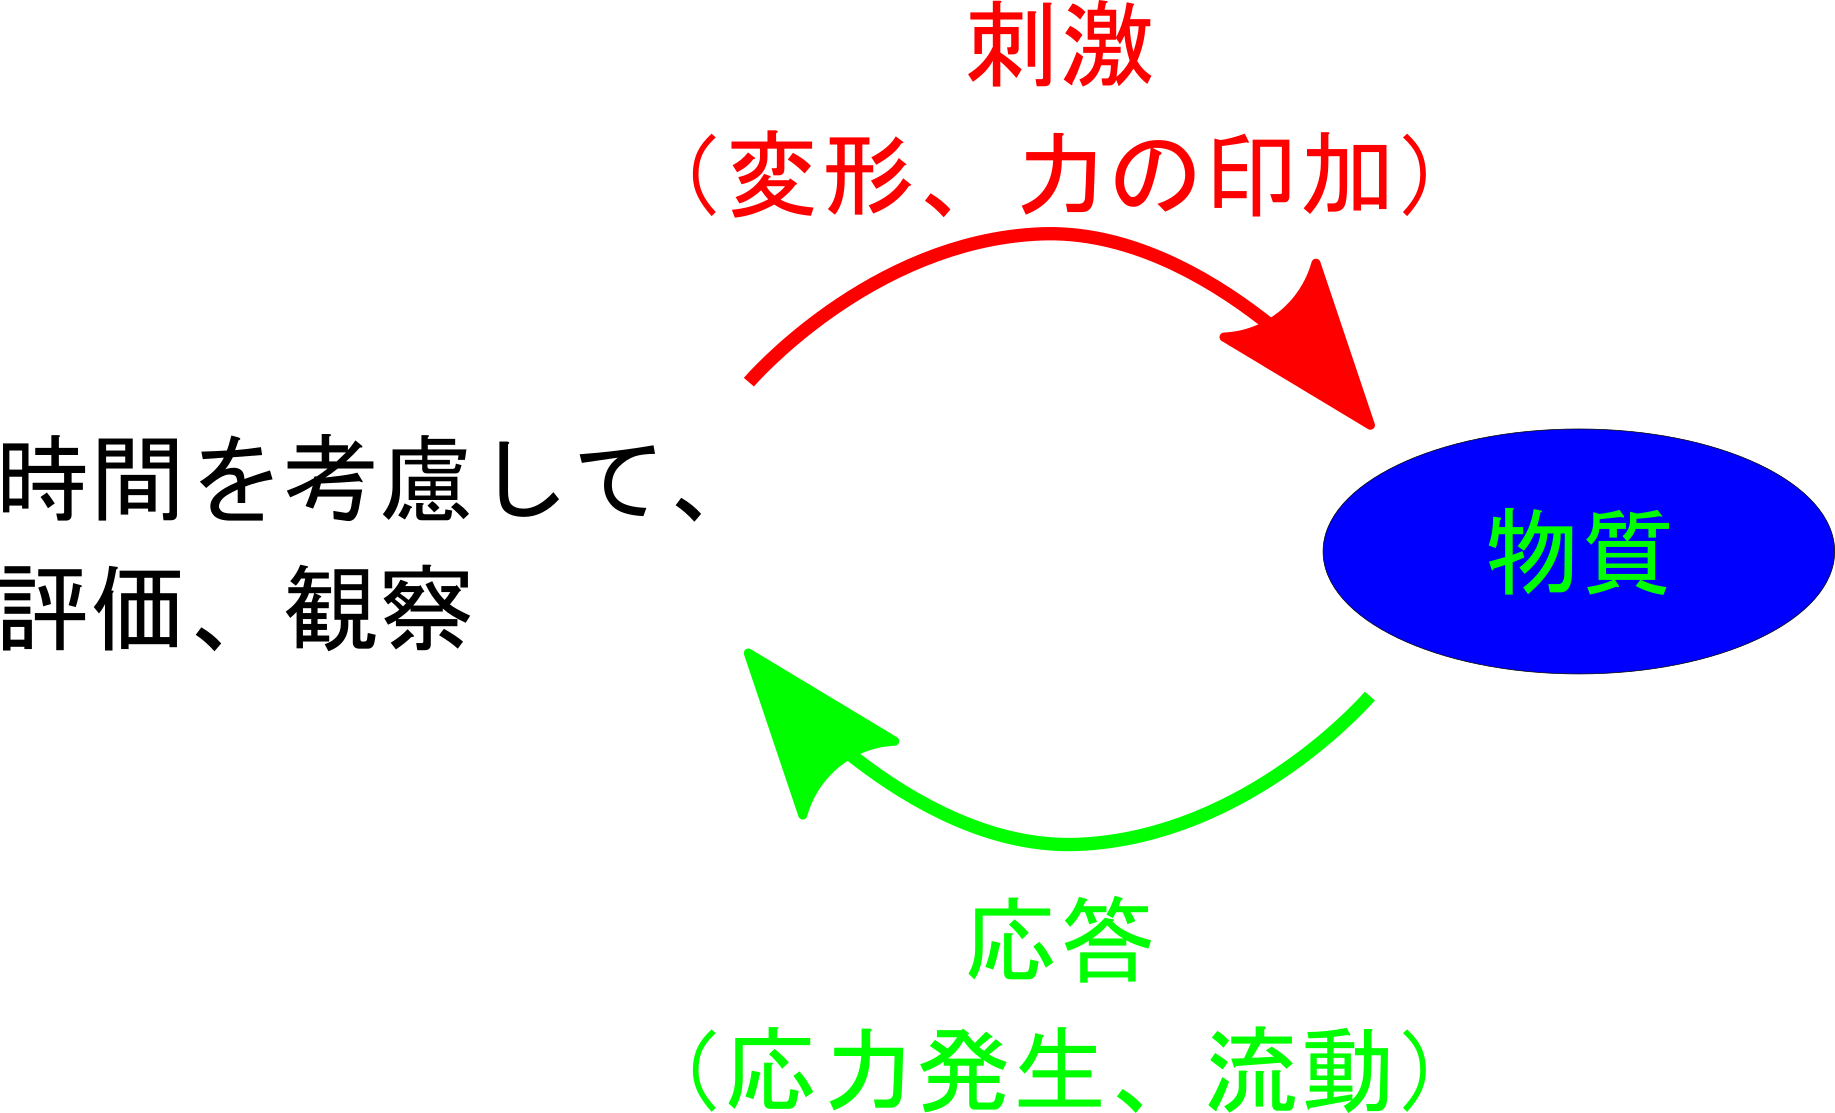
\includegraphics[width=\textwidth]{Rheo_method.png}
		\column{.38\linewidth}
			\begin{itemize}
				\item 力学的な刺激
				\begin{itemize}
					\item 外力による\\物質の変形
				\end{itemize}
				\item 変形の結果として
				\begin{itemize}
					\item 応力が発生
				\end{itemize}
				\item 弾性と粘性
			\end{itemize}
	\end{columns}
\end{frame}

% \begin{frame}
% 	\frametitle{固体と液体の応答について}
% 			\begin{center}
% 				\begin{tabular}{|c||c|} \hline
% 					固体のモデル	& 液体のモデル \\ \hline \hline
% 					応力は\alert{ひずみに比例}	& 応力は\alert{ひずみ速度に比例}\\
% 					$\text{応力} = \text{弾性率} \times \text{ひずみ}$	& $\text{応力} = \text{粘度} \times \text{ひずみ速度}$ \\ \hline
% 					比例定数が弾性率	& 比例定数が粘度\\ 
% 					弾性率の単位は、[Pa]	& 粘度の単位は、[Pa$\cdot$s]\\ \hline
% 					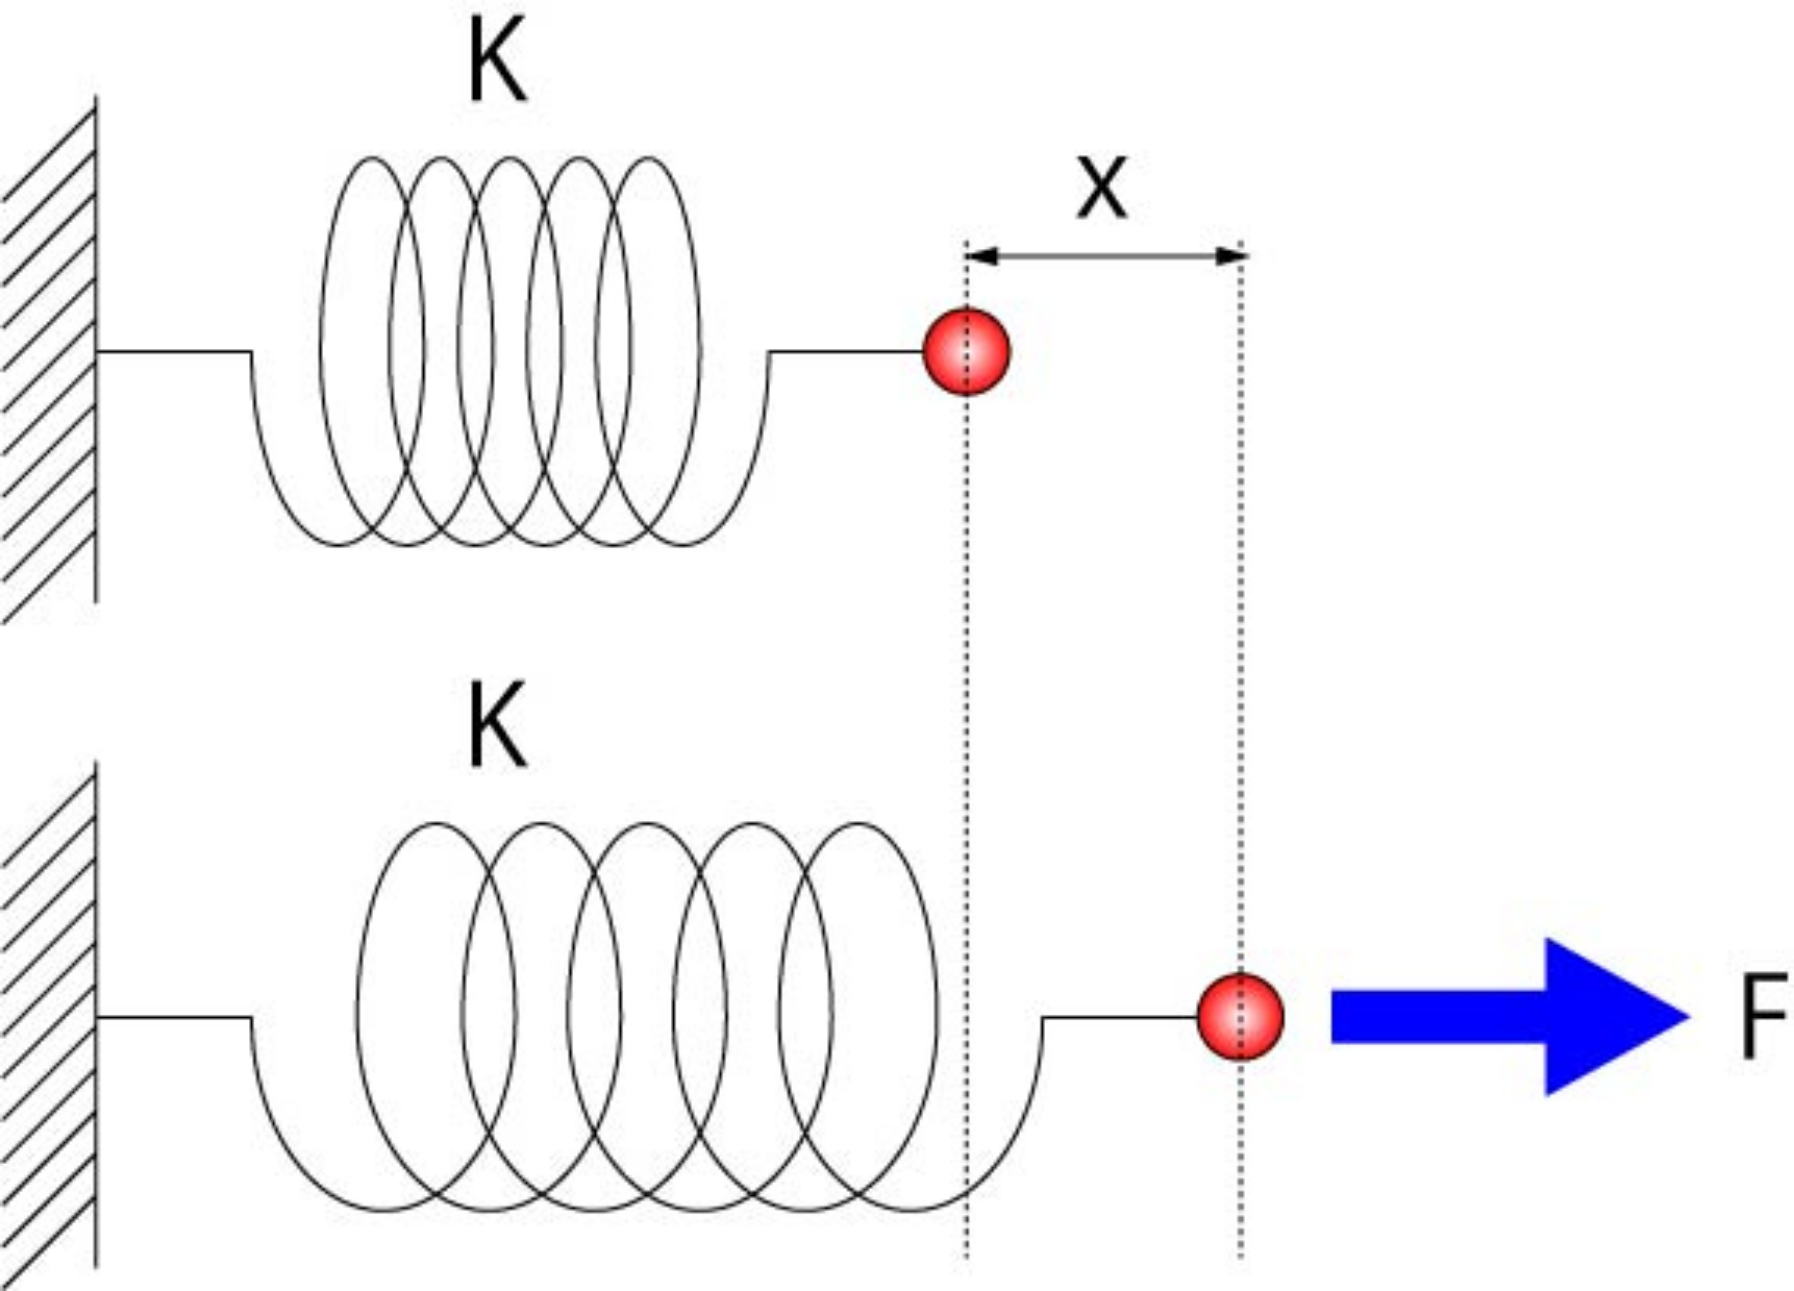
\includegraphics[width= 0.25\textwidth]{spring.png} & 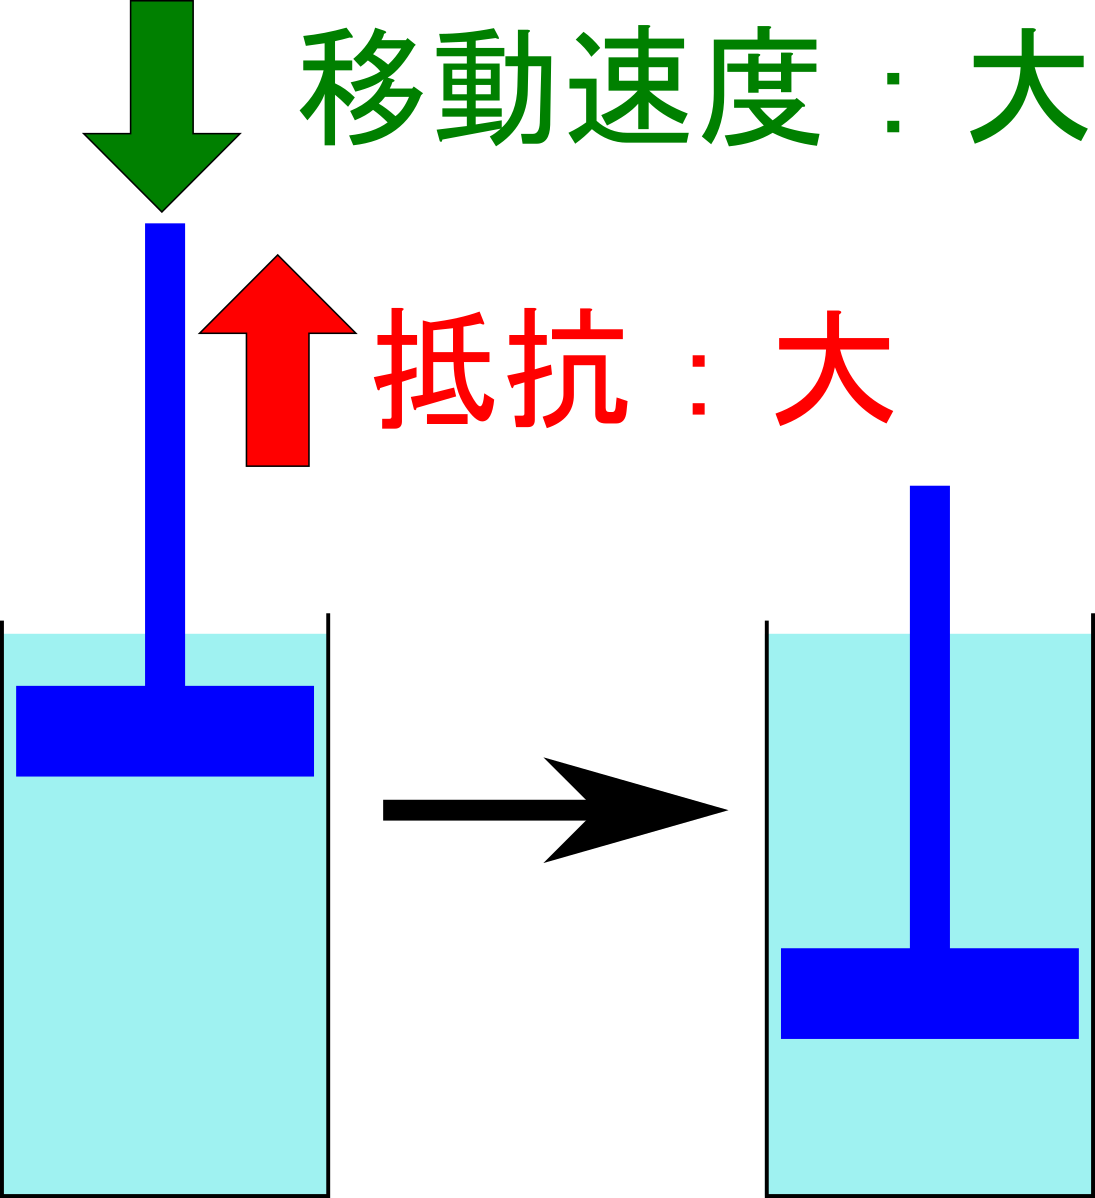
\includegraphics[width=.25\textwidth]{dashpot.png} \\ \hline
% 					\alert{力の釣り合い}	& 	\alert{時間の因子が重要} \\ \hline
% 				\end{tabular}
% 			\end{center}
% \end{frame}

% \begin{frame}
% 	\frametitle{各種の応答特性の分類}
% 		\begin{itemize}
% 			\item 図の左側が弾性応答
% 			\item 右側が流動特性
% 			\item 単純に二分されるわけでもなく、\alert{粘性と弾性を\\併せ持ったもの}が多く存在。
% 		\end{itemize}
% 			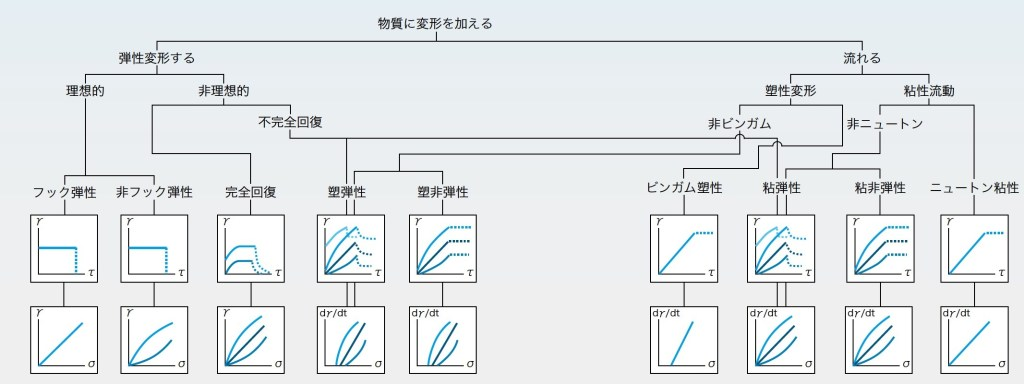
\includegraphics[width=\textwidth]{reoroji.jpeg}
% 			Nature 1942 v149-3790, p702
% 			% \href{http://rheology.jp/nagoya/2017/10/%e3%83%ac%e3%82%aa%e3%83%ad%e3%82%b8%e3%83%bc%e7%9a%84%e3%81%aa%e7%89%a9%e8%b3%aa%e3%81%ae%e5%88%86%e9%a1%9e/}{この絵のサイトへのリンク}
% \end{frame}

% \subsection{粘弾性のモデル化}
% \begin{frame}
% 	\frametitle{粘弾性について}
% 		\begin{block}{粘弾性とは?}
% 			\begin{itemize}
% 				\item 液体の流れる性質「粘性」と、
% 				\item 固体の変形する性質「弾性」を
% 				\item 合わせ持つ複雑な性質が、
% 				\item 「粘弾性」という事になります
% 			\end{itemize}
% 		\end{block}
% 		\begin{exampleblock}{単純に考えて、}
% 			\begin{itemize}
% 				\item 弾性を表すバネを用いたモデル
% 				\item 粘性を表すダッシュポットを用いたモデル
% 				\item 2つを組み合わせたモデル
% 			\end{itemize}
% 		\end{exampleblock}
% \end{frame}

% \begin{frame}
% 	\frametitle{マックスウェルモデル}
% 		\begin{columns}[T, onlytextwidth]
% 			\column{.58\linewidth}
% 				\begin{block}{マックスウェルモデルとは}
% 					\begin{itemize}
% 						\item 弾性を表すバネと、
% 						\item 粘性を表すダッシュポットを、
% 						\item 直列に連結したモデル。
% 						\item 外部からの刺激に対して、
% 						\item それぞれのユニットが、\\錬成して応答
% 					\end{itemize}
% 				\end{block}
% 			\column{.38\linewidth}
% 				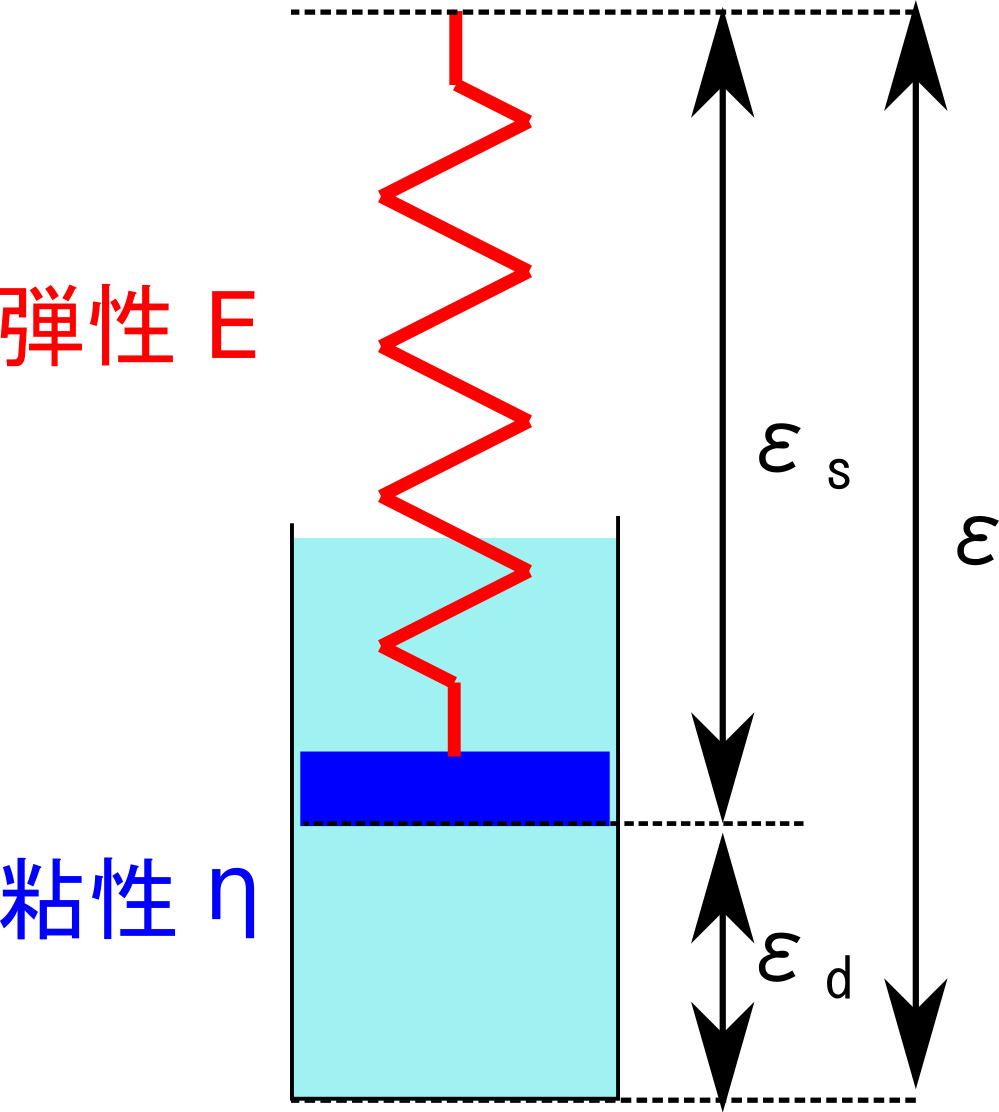
\includegraphics[width=\textwidth]{Maxwell_model.png}
% 		\end{columns}
% \end{frame}

% \subsection{粘弾性の応答}
% \begin{frame}
% 	\frametitle{粘弾性における応力緩和}
% 		\begin{columns}[T, onlytextwidth]
% 			\column{.48\linewidth}
% 				\begin{block}{マクロには}
% 					\begin{itemize}
% 						\item 物質にひずみを与えて、
% 						\item その状態に維持。
% 						\item 応力がしだいに減少。
% 					\end{itemize}
% 				\end{block}
% 			\column{.48\linewidth}
% 			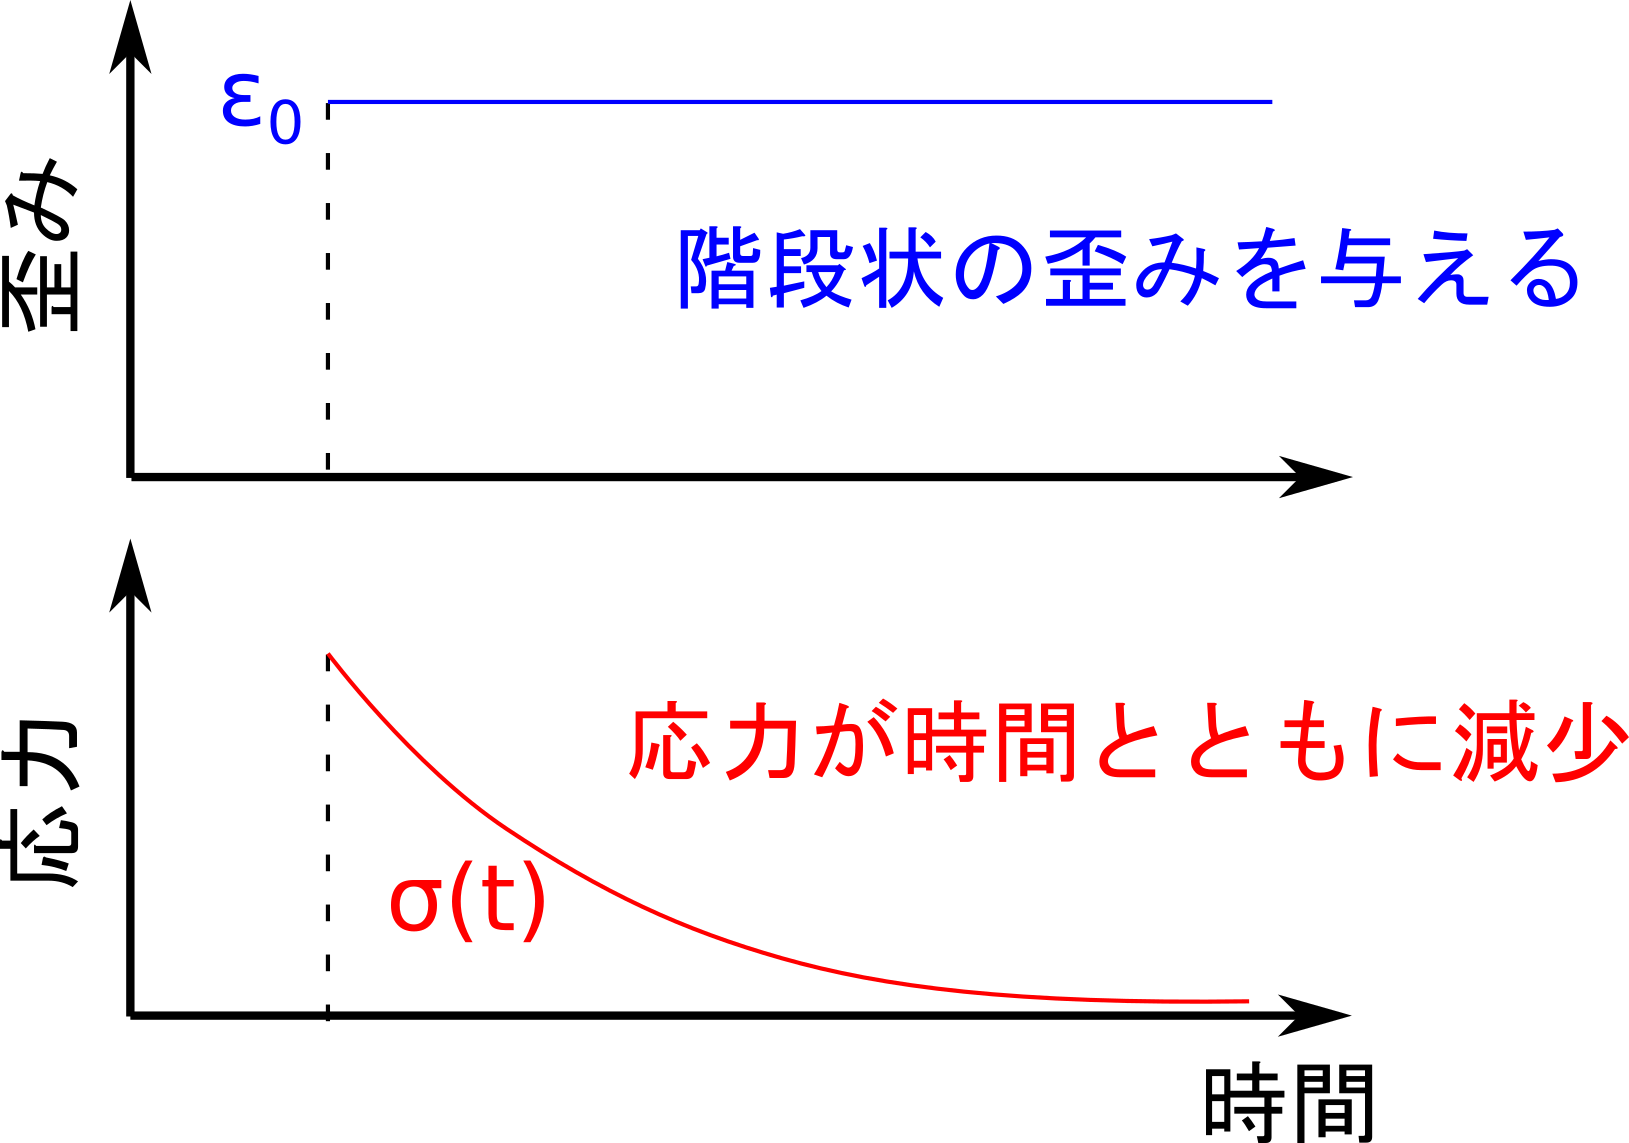
\includegraphics[width=\textwidth]{stress_relux.png}
% 		\end{columns}
		
% 		\begin{exampleblock}{ミクロには}
% 			\begin{itemize}
% 				\item 居心地のいい状態にいた粒子が、突然、居心地が変化。
% 				\item 少しずつ、\alert{居心地を改善}していく。
% 				\item 局所的な応力が消失。
% 			\end{itemize}
% 		\end{exampleblock}
% \end{frame}

% \begin{frame}
% 	\frametitle{応力緩和の挙動}
% 		\begin{columns}[T, onlytextwidth]
% 			\column{.48\linewidth}
% 				\begin{exampleblock}{指数関数的減少とは?}
% 					\begin{itemize}
% 						\item 下式をグラフに表すと、右図となる。
% 						\begin{align*}
% 							\sigma(t) = \sigma_0 \exp \left(-\dfrac{t}{\tau} \right)
% 						\end{align*}
% 						\item 時間経過に伴い応力が減少し $t = \tau$ において
% 						\begin{align*}
% 							\sigma(\tau) 
% 							&= \sigma_0 \exp(-1)\\ 
% 							&= \dfrac{\sigma_0}{e}
% 						\end{align*}
% 					\end{itemize}
% 				\end{exampleblock}
% 			\column{.48\linewidth}
% 				\begin{alertblock}{緩和時間とは、}
% 					時間の次元を持つ $\tau$ は、初期の $\dfrac{1}{e}$ となる時間
% 				\end{alertblock}
% 				\begin{center}
% 					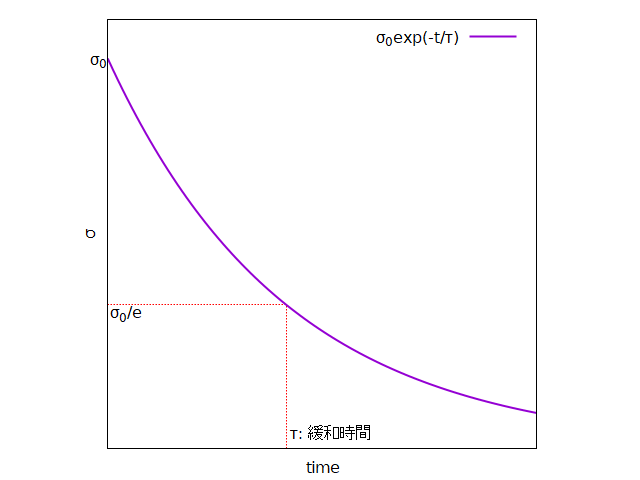
\includegraphics[width=\textwidth]{relux_3.png}
% 				\end{center}
% 		\end{columns}
% \end{frame}

% \begin{frame}
% 	\frametitle{緩和時間}
% 		\begin{align*}
% 			\text{(緩和時間)}\;\tau = \dfrac{\eta}{E}\; \left( \dfrac{\text{粘度}}{\text{弾性率}} \right)
% 		\end{align*}
% 		\vspace{-3mm}
% 		\begin{itemize}
% 			\item 緩和時間とは
% 			\begin{itemize}
% 				\item 弾性モデルにおける弾性率 $E$ の単位は Pa
% 				\item 粘性モデルにおける粘度 $\eta$ の単位は Pa$\cdot$s
% 				\item \alert{その比となる $\tau$ は時間の次元 [T] を持ち\\緩和時間}と呼ばれます
% 				\item 緩和時間とは、物質のひずみに対する力学応答が\\指数関数的に減少するさまを表す特徴的な時間。
% 			\end{itemize}
% 			\item 緩和時間の振る舞い
% 			\begin{itemize}
% 				\item 弾性応答の性質を表す\alert{弾性率に反比例}し
% 				\item 粘性応答の度合いを表す\alert{粘度に比例}します
% 			\end{itemize}
% 		\end{itemize}
% \end{frame}

% \begin{frame}
% 	\frametitle{粘弾性についてのまとめ}
%         \begin{boxnote}
%             \vspace{-3mm}
%             \begin{itemize}
%                 \item 粘性と弾性についての再確認
%                     \begin{itemize}
%                         \item 固体のモデルはバネ、液体はダッシュポット
%                         \item 液体の粘性は「時間の因子が重要」
%                     \end{itemize} 
%                 \item 粘弾性のモデル化
%                     \begin{itemize}
%                         \item 多くの物質は粘性と弾性を併せ持つ。
%                         \item 粘弾性のモデルはバネとダッシュポットを\\直列したマックスウェルモデル
%                     \end{itemize} 
%                 \item 粘弾性の応答
%                     \begin{itemize}
%                         \item ひずみを付与した応力緩和が特徴的
%                         \item 緩和現象は緩和時間で説明できる。
%                     \end{itemize}
%             \end{itemize}
%         \end{boxnote}
% \end{frame}

% \section{粘弾性体の動的な刺激への応答}
% \subsection{動的な刺激への応答}
% \begin{frame}
% 	\frametitle{動的な刺激に対する応答}
% 	\begin{itemize}
% 		\item 刺激を加えて、その応答を評価する。
% 		\item 今回は、\textcolor{red}{「動的な刺激」}を与える。
% 	\end{itemize}

% 	\vspace{5mm}
% 			\centering
% 				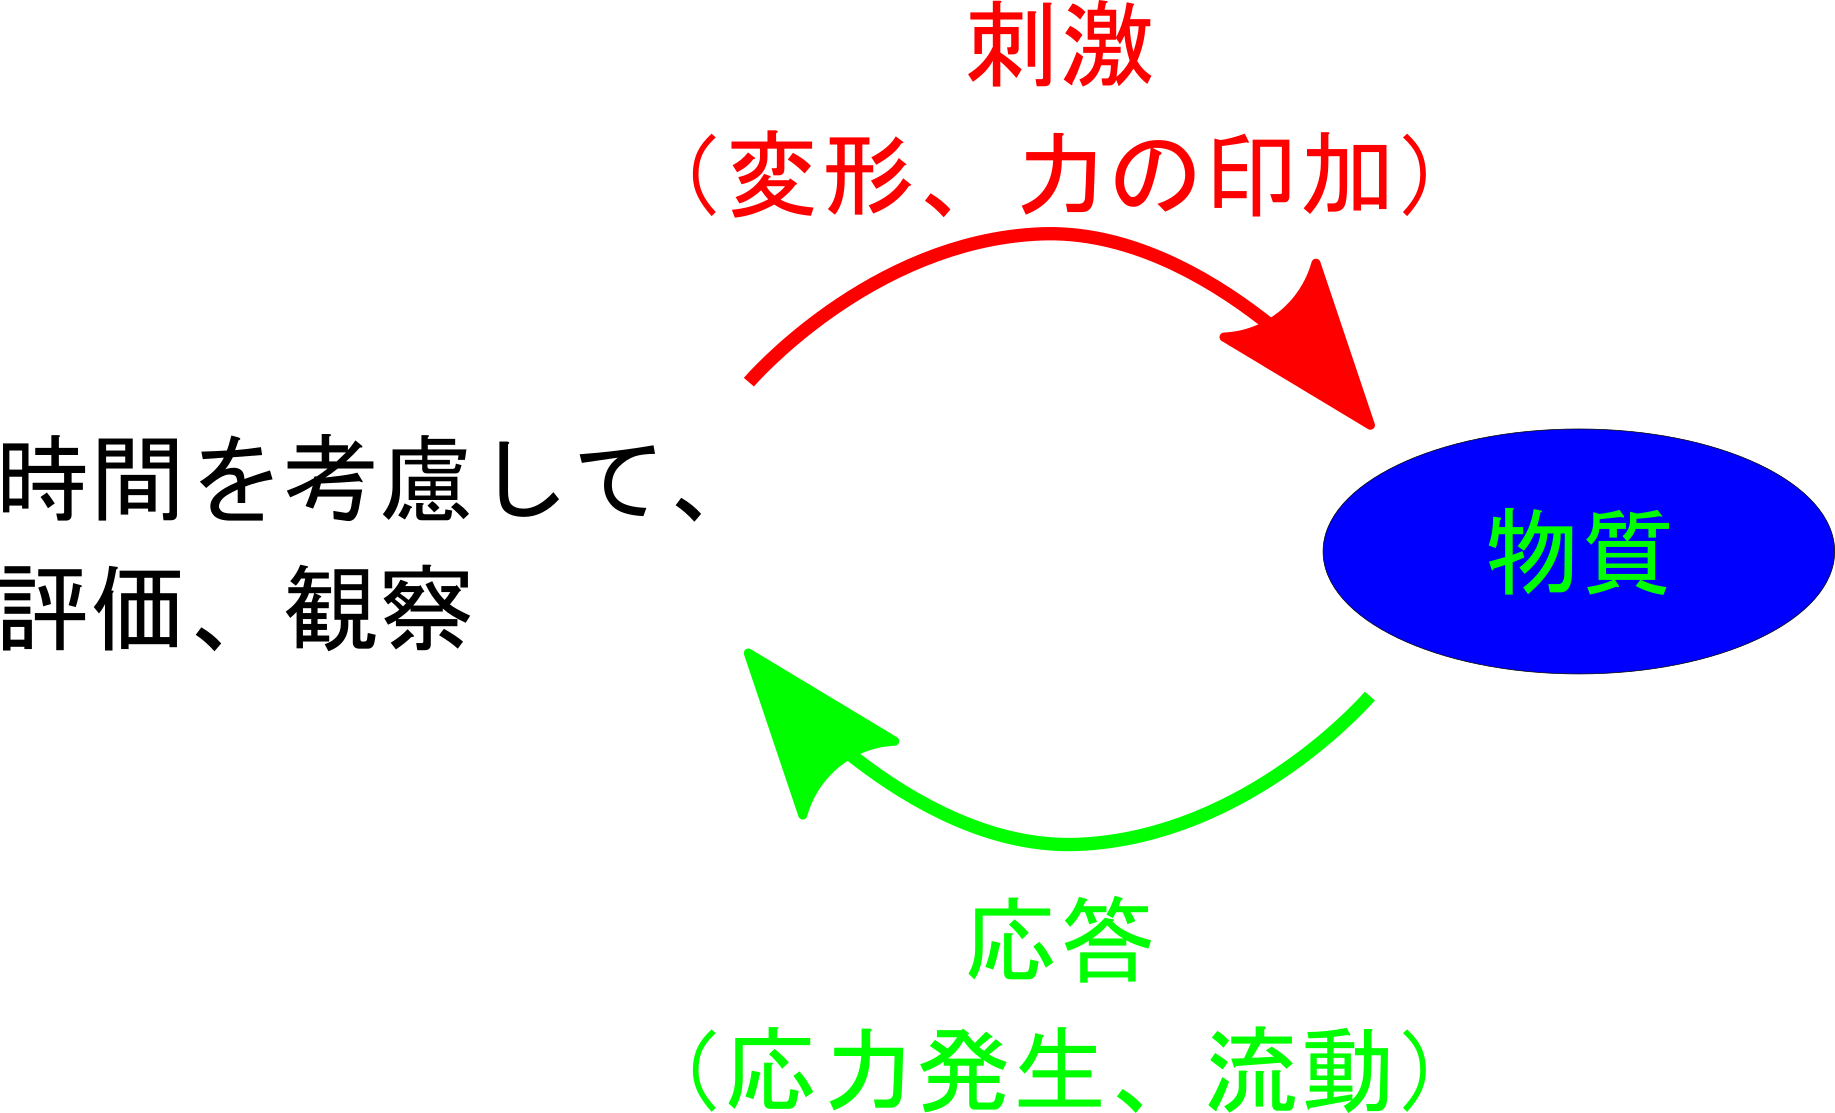
\includegraphics[width=.75\textwidth]{Rheo_method.png}
% \end{frame}

% \begin{frame}{周期的な入力のイメージ}
% 	\begin{exampleblock}{円運動 $\Leftrightarrow$ 単振動 $\Leftrightarrow$ 波動は等価}
% 		以下は、$\sin(\omega t)$ 等の三角関数の組み合わせで記述できる。

% 		\vspace{3mm}
% 		\centering
% 		\animategraphics[loop, width=0.75\textwidth, autoplay]{20}{vibration/vibration-}{0}{50}
% 	\end{exampleblock}
% \end{frame}

% \begin{frame}
% 	\frametitle{動的な刺激について}
% 	\begin{block}{動的なひずみとは?}
% 		\begin{itemize}
% 			\item 周期(繰り返し)的に時間変化するひずみ $\gamma (t)$\\
% 			$\gamma (t) = \gamma_0 \sin(\omega t)$
% 			\item $\omega$ は角周波数で、回転速度を表すスカラー量\\
% 			$\omega \equiv \dfrac{\mathrm{d} \theta}{\mathrm{d} t} = \dfrac{2 \pi}{T} = 2\pi f$
% 			\begin{itemize}
% 				\item $\theta$ は角度 (単位:ラジアン)
% 				\item $T$ は周期 (単位:秒)
% 				\item $f$ は周波数 (単位:ヘルツ)
				
% 			\end{itemize}
% 			\item 角周波数 $\omega$ について
% 			\begin{itemize}
% 				\item $\theta$ が無次元量であるので、$\omega$ の次元は $T^{-1}$
% 				\item SI 単位は、ラジアン毎秒 (rad/s)
% 				\item 角周波数は通常の周波数を単純に $2\pi$ 倍したもの
% 			\end{itemize}
% 		\end{itemize}
% 	\end{block}

% \end{frame}

% % \subsection{動的な応答を評価する}
% \begin{frame}
% 	\frametitle{動的な応答を評価する。}
% 		\begin{block}{動的な刺激と応答の評価}
% 			\begin{itemize}
% 				\item 入力したひずみに対応して出力する応力を評価
% 				\begin{itemize}
% 					\item 入力:周期的な変形 $\gamma(t) = \gamma_0 \sin(\omega t)$
% 					\item 出力:変形に対応した応力 $\sigma(t)$
% 				\end{itemize}
% 				\item 付与した刺激 $\gamma (t)$ と出力した応答 $\sigma (t)$ を比べる。
% 				\begin{itemize}
% 					\item 同軸上に並べて比べる。
% 					\item 直交する形で評価する。⇒ Lissajous 曲線
% 				\end{itemize}
% 				\item 粘弾性測定の場合は、入力と出力の周期は同一。
% 			\end{itemize}
% 		\end{block}
% 		\vspace{3mm}
% 		\centering
% 			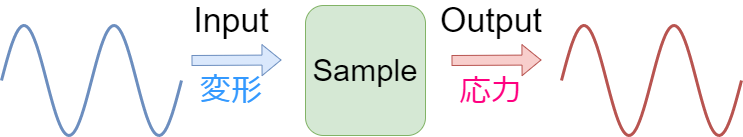
\includegraphics[width=\textwidth]{dynamic_IO.png}
% \end{frame}

% \begin{frame}
% 	\frametitle{Lissajous 曲線}
% 		\begin{block}{リサジュー曲線 (Lissajous curve)とは?}
% 			\begin{itemize}
% 				\item 互いに直交する二つの単振動を合成した平面図形。
% 				\begin{itemize}
% 					\item 一般に入力を x 軸、出力を y 軸
% 					\item オシロスコープでの周波数測定に用いられる。
% 					\item 入出力信号の位相が安定しないと変化を繰り返す。
% 				\end{itemize}
% 				\item “リサージュ”と表記されることもある。
% 				\item \textcolor{red}{\href{https://ja.wikipedia.org/wiki/リサジュー図形}{「リサジュー図形」のWiki}}へのリンク
% 			\end{itemize}
% 		\end{block}

% 	\begin{columns}[c, onlytextwidth]
% 		\column{.15\linewidth}
% 		\column{.25\linewidth}
% 				\centering
% 					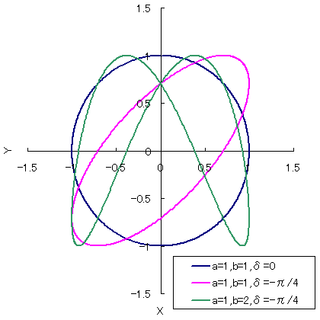
\includegraphics[width=\textwidth]{Lissajou.png}	
% 		\column{.5\linewidth}
% 			\begin{itemize}
% 				\item 安定した出力の例
% 			\end{itemize}
% 			\vspace{-5mm}
% 			\begin{align*}
% 				x&=A \cos(at) \\
% 				y&=B \sin(bt + \delta)
% 			\end{align*}
% 		\column{.1\linewidth}	
% 	\end{columns}
% \end{frame}


% \begin{frame}
% 	\frametitle{位相とは?}
% 		\begin{block}{位相とは?}
% 			\begin{itemize}
% 				\item 周期的に変動する波の位置情報を意味します。
% 				\begin{itemize}
% 					\item 入力信号が正弦波 $A \sin (\omega t + \phi)$ で表されたとき、
% 					\item 入力を表す変数(角度)$\omega t + \phi$ を指します。
% 					\item ここで、$t=0$ の時の位相 $\phi$ を初期位相と呼びます。
% 				\end{itemize}
% 				\item ちなみに、正弦波の一般式 $A \sin (\omega t + \phi)$ において、\\
% 				振幅:$A$、角周波数:$\omega$、初期位相:$\phi$ となる。
% 			\end{itemize}
% 		\end{block}

% 		\begin{alertblock}{異なる波の位相を比較する場合、}
% 			\begin{itemize}
% 				\item 一方が $A \sin (\omega_A t + \phi_A)$、他方が $B \sin (\omega_B t + \phi_B)$  
% 				\item 初期位相($\phi_A, \phi_B$)の差 $\Delta \phi = \phi_B - \phi_A$ で評価
% 				\item $\Delta \phi$ が正の場合を位相進み、負を位相遅れと呼ぶ。
% 			\end{itemize}
% 		\end{alertblock}
% \end{frame}

% \subsection{理想的な弾性固体や粘性液体の応答}

% \begin{frame}
% 	\frametitle{固体と液体の応答について}
% 			\begin{center}
% 				\begin{tabular}{|c||c|} \hline
% 					固体のモデル	& 液体のモデル \\ \hline \hline
% 					応力は\alert{ひずみに比例}	& 応力は\alert{ひずみ速度に比例}\\
% 					$\text{応力} = \text{弾性率} \times \text{ひずみ}$	& $\text{応力} = \text{粘度} \times \text{ひずみ速度}$ \\ \hline
% 					比例定数が弾性率	& 比例定数が粘度\\ 
% 					弾性率の単位は、[Pa]	& 粘度の単位は、[Pa$\cdot$s]\\ \hline
% 					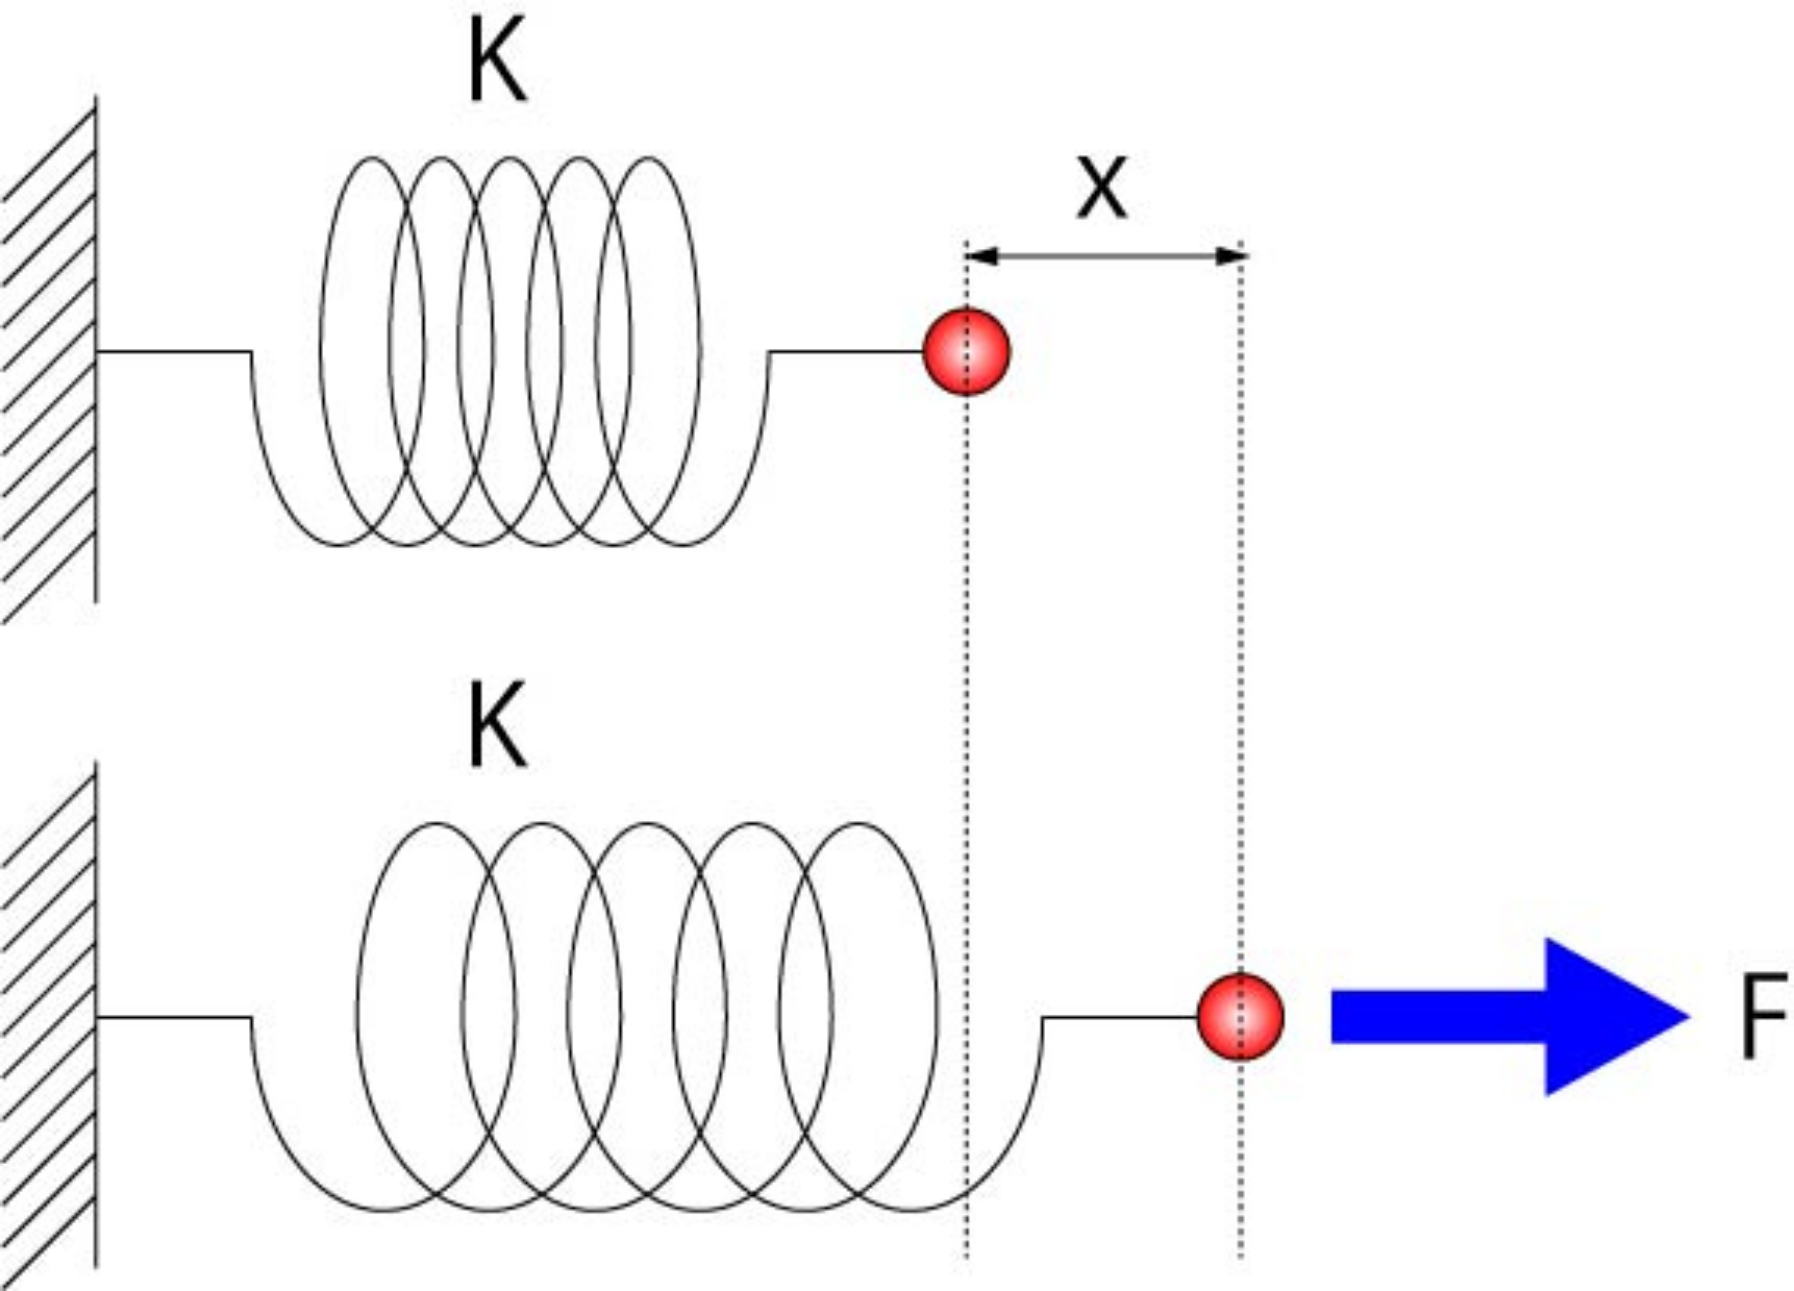
\includegraphics[width= 0.25\textwidth]{spring.png} & 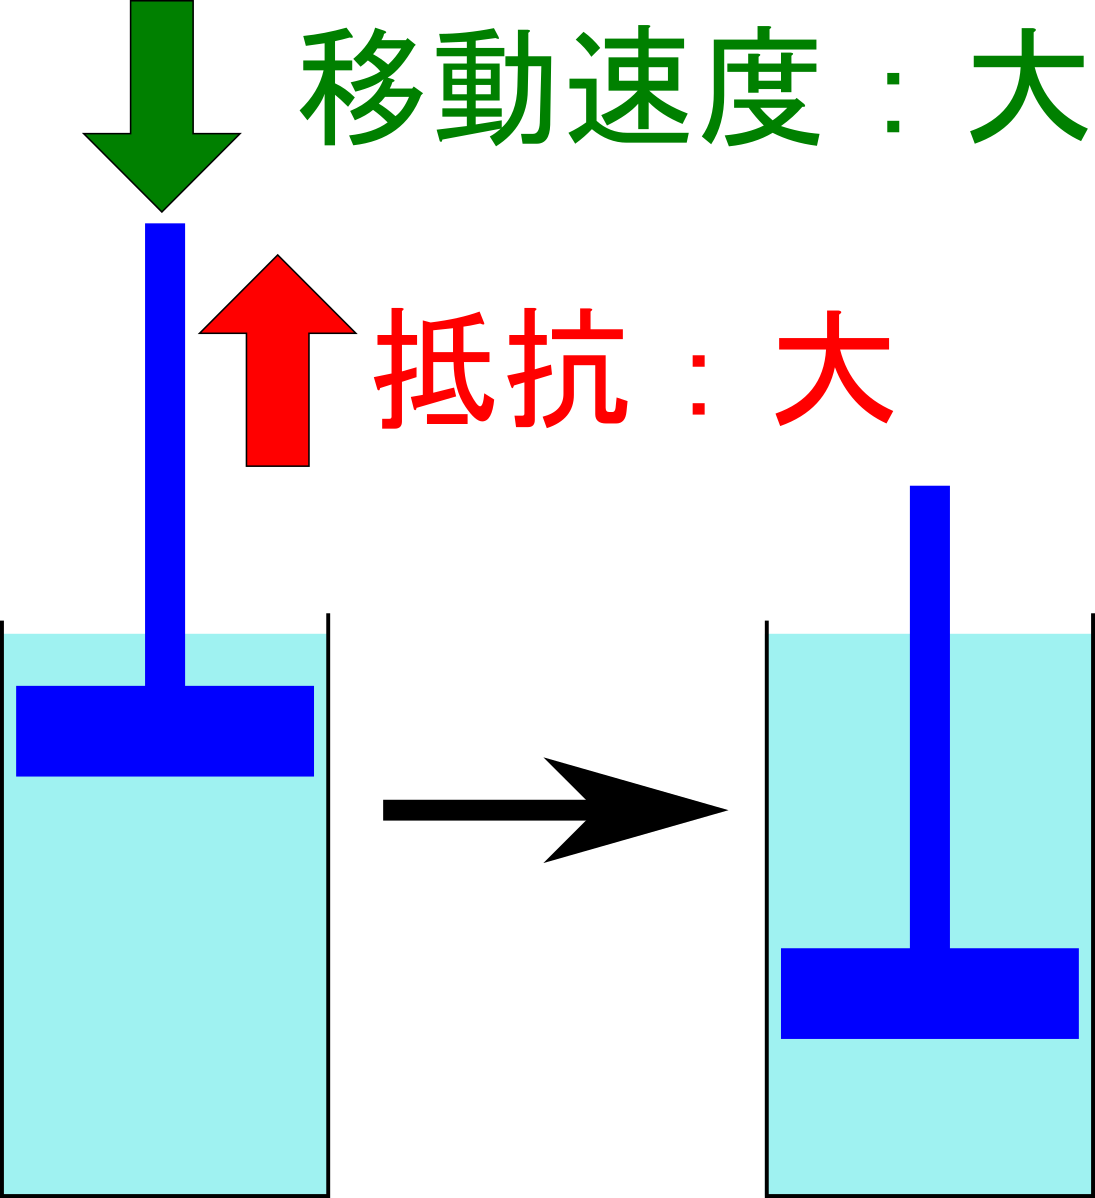
\includegraphics[width=.25\textwidth]{dashpot.png} \\ \hline
% 					\alert{力の釣り合い}	& 	\alert{時間の因子が重要} \\ \hline
% 				\end{tabular}
% 			\end{center}
% \end{frame}

% \begin{frame}
%     \frametitle{理想的な弾性固体の応答}
% 	\begin{block}{弾性固体に周期的な変形を印加}
% 		\begin{itemize}
% 			\item 弾性固体のモデル:バネ
% 			\item 周期的な変形を入力 $\Leftrightarrow$ 同位相の応力が出力\\
% 			$\text{入力:}\gamma (t) = \gamma_0 \sin(\omega t) \Leftrightarrow \text{出力:}\sigma = \sigma_0 \sin(\omega t)$
% 		\end{itemize}
% 	\end{block}
% 	\begin{columns}[c, onlytextwidth]
% 		\column{.38\linewidth}
% 			\centering
% 				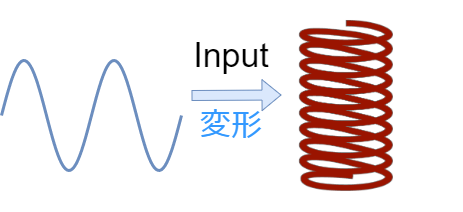
\includegraphics[width=\textwidth]{dynamic_Elast.png}
			
% 		\column{.6\linewidth}
% 			\centering
% 				\animategraphics[loop, width=\textwidth, autoplay]{20}{dynamic_rheo_elast/dyn_rheo_elast-}{0}{50}
% 	\end{columns}
% \end{frame}

% \begin{frame}
%     \frametitle{理想的な弾性固体の応答}
% 	\begin{block}{Lissajous 曲線から}
% 		\begin{itemize}
% 			\item 入力ひずみと出力応力が比例
% 			\item 比例定数が弾性率 $G$ 
% 		\end{itemize}
% 	\end{block}

% 		\centering
% 			\animategraphics[loop, width=.7\textwidth, autoplay]{20}{dynamic_rheo_elast/dyn_rheo_elast-}{0}{50}
% \end{frame}


% \begin{frame}
%     \frametitle{理想的な粘性液体の応答}
% 		\begin{block}{粘性液体に周期的な変形を印加}
% 			\begin{itemize}
% 				\item 粘性液体のモデル:ダッシュポット
% 				\item 周期的な変形を入力 $\Leftrightarrow$ 位相が $\dfrac{\pi}{2}$ 進んだ応力が応答\\
% 				$\text{入力:}\gamma (t) = \gamma_0 \sin(\omega t) \Leftrightarrow \text{出力:}\sigma(t) = \sigma_0 \sin(\omega t + \dfrac{\pi}{2})$
% 				% \item 弾性率に応じて応力が変化
% 			\end{itemize}
% 		\end{block}
% 		\begin{columns}[c, onlytextwidth]
% 			\column{.38\linewidth}
% 				\centering
% 					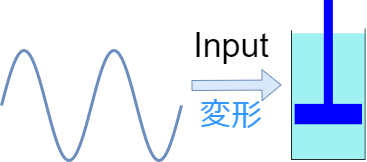
\includegraphics[width=\textwidth]{dynamic_Visco.png}
				
% 			\column{.6\linewidth}
% 				\centering
% 					\animategraphics[loop, width=\textwidth, autoplay]{20}{dynamic_rheo_visco/dyn_rheo_visco-}{0}{50}
% 		\end{columns}
% \end{frame}

% \begin{frame}
%     \frametitle{理想的な粘性液体の応答}
% 		\begin{block}{粘性液体に周期的な変形を印加}
% 			\begin{itemize}
% 				\item 出力応力はひずみ速度に比例 $\; \Rightarrow \; \sigma (t) \propto \dot{\gamma}(t) = \odv*{\gamma (t)}{t} $
% 				\item ひずみ速度はひずみの時間微分 \\
% 				$\Rightarrow \odv*{\gamma(t)}{t} = \odv*{\gamma_0 \sin(\omega t)}{t} = \gamma_0 \omega \cos(\omega t)$
% 				\item 出力応力とひずみ速度は同位相で、比例定数が粘度 $\eta$
% 			\end{itemize}
% 		\end{block}

% 		\centering
% 			\animategraphics[loop, width=.6\textwidth, autoplay]{20}{dynamic_rheo_visco/dyn_rheo_visco2-}{0}{50}
% \end{frame}

% \subsection{粘弾性体の応答}
% \begin{frame}
% 	\frametitle{粘弾性体とマックスウェルモデル}
% 	\begin{itemize}
% 		\item 大半の固体は、弾性と粘性を併せ持つ。
% 		\item この粘弾性を表すモデルがマックスウェルモデル
% 	\end{itemize}
% 	\begin{columns}[c, onlytextwidth]
% 		\column{.36\linewidth}
% 		\centering
% 		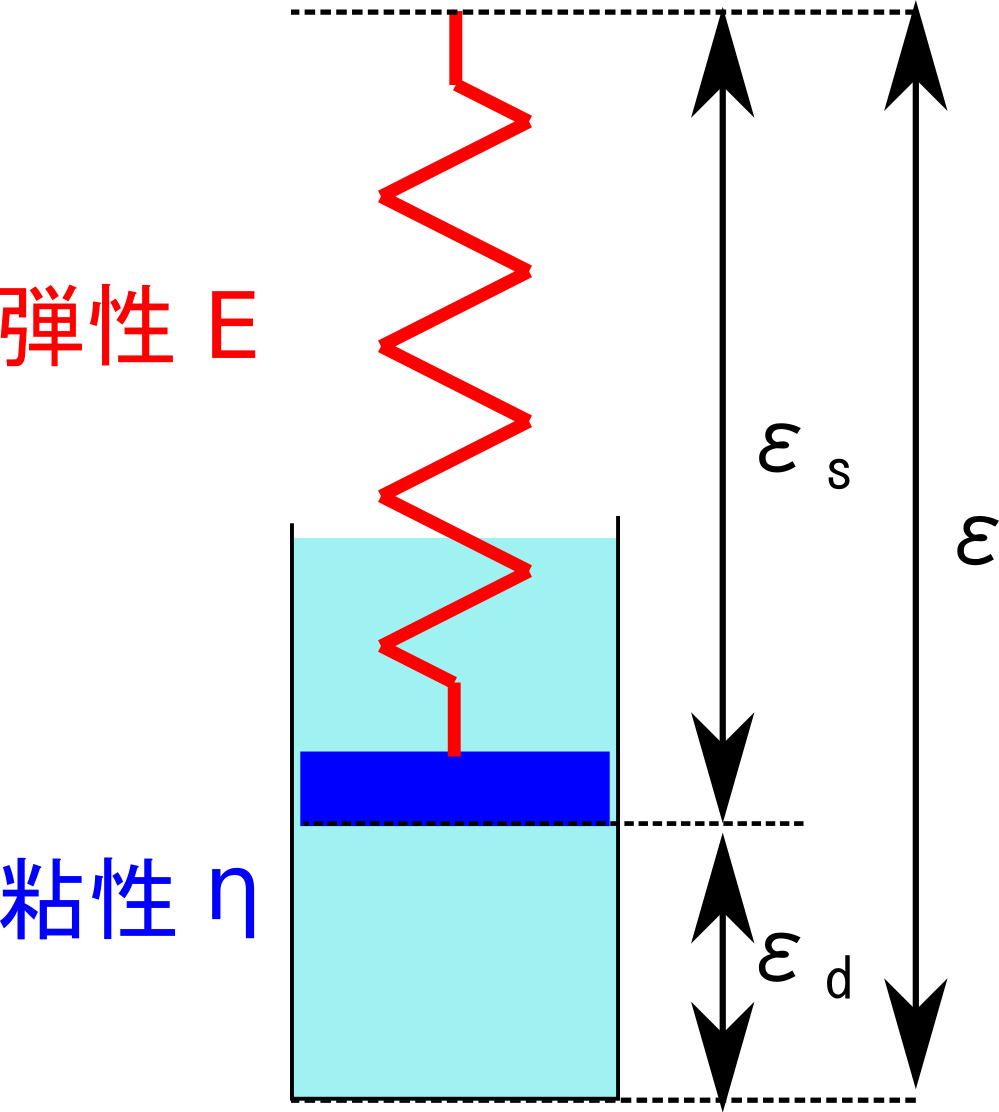
\includegraphics[width=.9\textwidth]{Maxwell_model.png}
% 		\column{.62\linewidth}
% 		\begin{block}{マックスウェルモデルとは}
% 			\begin{itemize}
% 				\item モデル構成
% 				\begin{itemize}
% 					\item 弾性を表すスプリングと、
% 					\item 粘性を表すダッシュポットを、
% 					\item 直列に連結したモデル。
% 				\end{itemize}
% 				\item 力学的な応答
% 				\begin{itemize}
% 					\item 外部からの刺激に対して、
% 					\item それぞれが錬成して応答。
% 				\end{itemize}
% 			\end{itemize}
			
% 		\end{block}
% 	\end{columns}
% \end{frame}

% \begin{frame}
%     \frametitle{粘弾性体の応答}
% 	\begin{block}{粘弾性体に周期的な変形を印加}
% 		\begin{itemize}
% 			\item 粘性液体のモデル:バネとダッシュポットの組み合わせ
% 			\item 周期的な変形を入力 $\Leftrightarrow$ 位相が $\delta$ 進んだ応力が応答\\
% 			$\text{入力:}\gamma (t) = \gamma_0 \sin(\omega t) \Leftrightarrow \text{出力:}\sigma(t) = \sigma_0 \sin(\omega t + \delta)$
% 		\end{itemize}
% 	\end{block}
% 	\begin{columns}[c, onlytextwidth]
% 		\column{.38\linewidth}
% 			\centering
% 				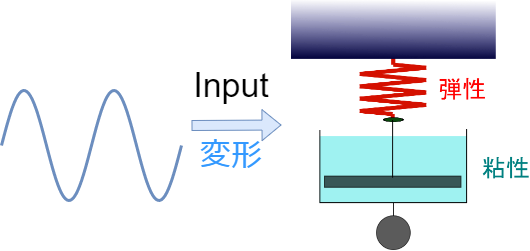
\includegraphics[width=\textwidth]{dynamic_ViscoElast.png}
			
% 		\column{.6\linewidth}
% 			\centering
% 				\animategraphics[loop, width=\textwidth, autoplay]{20}{dynamic_rheo_viscoelast/dyn_rheo_viscoelast-}{0}{50}
% 	\end{columns}
% \end{frame}

% % \subsection{粘弾性体の応答を分解する}
% \begin{frame}
% 	\frametitle{粘弾性体の応答を分解すると}
% 		\begin{block}{加法定理を用いて分解すると}
% 			\begin{itemize}
% 				\item 加法定理は以下、\\$A \sin(x + B) = A \sin(x) \cos(B) + A \cos(x) \sin(B)$
% 				\item このとき、入力 $\gamma_0 \sin(\omega t)$ への応答 $\sigma_0 \sin(\omega t + \delta)$ は、
% 				\begin{itemize}
% 					\item \textcolor{red}{入力と同位相の弾性応答} と 
% 					\item \text{\textcolor{blue}{$\dfrac{\pi}{2}$ 位相の進んだ粘性応答}}に分解できる。
% 				\end{itemize}
% 			\end{itemize}
% 		\end{block}
		
% 		\vspace{-7mm}
% 		\begin{align*}
% 			\sigma(t) &= \sigma_0 \sin(\omega t + \delta) \\
% 			&= \sigma_0 \sin(\omega t) \cos(\delta) + \sigma_0 \cos(\omega t) \sin(\delta) \\
% 			&= \underbrace{\overbrace{\sigma_0 \cos(\delta)}^{\text{\textcolor{red}{弾性由来の応力}}} \sin(\omega t)}_{\text{\textcolor{red}{入力と同位相の弾性応答}}} 
% 			+ \underbrace{\overbrace{\sigma_0 \sin(\delta)}^{\text{\textcolor{blue}{粘性由来の応力}}} \sin(\omega t + \dfrac{\pi}{2})}_{\text{\textcolor{blue}{$\dfrac{\pi}{2}$ 位相の進んだ粘性応答}}} 
% 		\end{align*}

% \end{frame}

% \begin{frame}
%     \frametitle{弾性的な応答を表す貯蔵弾性率 $G^{\prime}$}
		
% 		\begin{alertblock}{貯蔵弾性率 $G^{\prime}$}
% 			\begin{itemize}
% 				\item ひずみ $\gamma(t)$ と位相の揃った弾性的な応答応力 $\sigma_e(t)$ は、\\
% 				$\sigma_e(t) = \sigma_0 \cos(\delta)\sin(\omega t)$
% 				\item この弾性由来の応力をひずみ量で除して、
% 				\item 弾性的な応答に対応する\textcolor{red}{貯蔵弾性率 $G^{\prime}$}
% 			\end{itemize}
% 			\begin{columns}[c, onlytextwidth]
% 				\column{.55\linewidth}
% 						\begin{align*}
% 							G^{\prime} &= \dfrac{\text{弾性由来の応力}}{\text{ひずみ量}} \\
% 							&= \dfrac{\sigma_0 \cos(\delta)}{\gamma_0}
% 						\end{align*}
% 				\column{.45\linewidth}
% 					\centering
% 					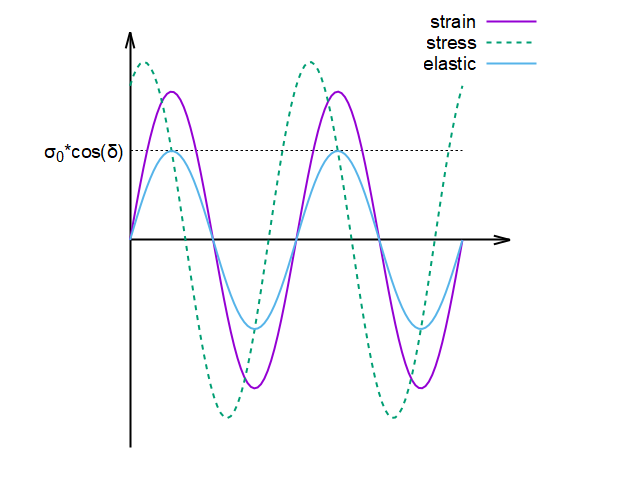
\includegraphics[width=\textwidth]{dynamic_rheo/dyn_rheo_ela.png}
% 			\end{columns}
% 		\end{alertblock}
% \end{frame}

% \begin{frame}
%     \frametitle{粘性的な応答を表す損失弾性率 $G^{\prime\prime}$}
		
% 		\begin{block}{損失弾性率 $G^{\prime\prime}$}
% 			\begin{itemize}
% 				\item ひずみ $\gamma(t)$ から $\dfrac{\pi}{2}$ 位相の進んだ粘性的な応答応力 $\sigma_v(t)$ は、
% 				$\sigma_v(t) = \sigma_0 \sin(\delta)\sin(\omega t + \dfrac{\pi}{2})$
% 				\item この粘性由来の応力をひずみ量で除して、
% 				\item 粘性的な応答に対応する\textcolor{red}{損失弾性率 $G^{\prime\prime}$}
% 			\end{itemize}
% 			\begin{columns}[c, onlytextwidth]
% 				\column{.55\linewidth}
% 						\begin{align*}
% 							G^{\prime \prime} &= \dfrac{\text{粘性由来の応力}}{\text{ひずみ量}} \\
% 							&= \dfrac{\sigma_0 \sin(\delta)}{\gamma_0}
% 						\end{align*}
% 				\column{.45\linewidth}
% 					\centering
% 					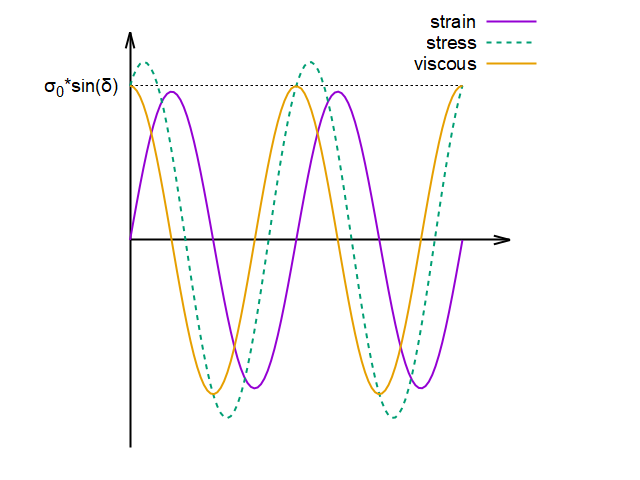
\includegraphics[width=.9\textwidth]{dynamic_rheo/dyn_rheo_visco.png}
% 			\end{columns}
% 		\end{block}
% \end{frame}


% \begin{frame}
%     \frametitle{損失正接 $\tan \delta$ とは?}
% 		\begin{block}{損失正接とは?}
% 			\begin{itemize}
% 				\item 粘性の寄与の度合いを表すものであり、
% 				\item 損失弾性率と貯蔵弾性率との比で定まる。
% 			\end{itemize}

% 			\begin{columns}[c, onlytextwidth]
% 				\column{.48\linewidth}
% 				\begin{align*}
% 					\dfrac{\text{損失弾性率}}{\text{貯蔵弾性率}} &= \dfrac{\sigma_0 \sin(\delta)/\gamma_0}{\sigma_0 \cos(\delta)/\gamma_0} \\
% 					&= \dfrac{\sin(\delta)}{\cos(\delta)} \\
% 					&= \tan(\delta)
% 				\end{align*}

% 				\vspace{-8mm}
% 				\begin{equation*}
% 					\tan(\delta)
% 					\begin{cases}
% 						> 1 &\text{粘性的} \\
% 						< 1 &\text{弾性的}
% 					\end{cases}
% 				\end{equation*}
% 				\column{.48\linewidth}
% 				\centering
% 				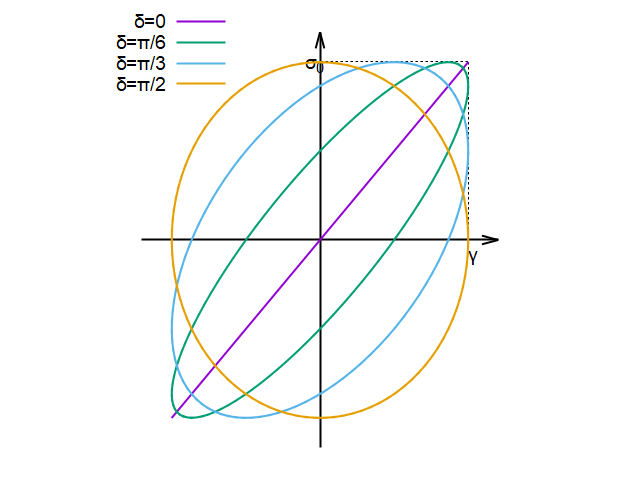
\includegraphics[width=\textwidth]{dynamic_rheo/dyn_rheo_lissajou.png}
% 			\end{columns}
% 		\end{block}
% \end{frame}

% % \subsection{動的粘弾性測定とは}
% \begin{frame}
% 	\frametitle{動的粘弾性測定とは}

% 		\vspace{-5mm}
% 	\begin{columns}[T, onlytextwidth]
% 		\column{.38\linewidth}
% 			\begin{exampleblock}{変更可能なパラメタ}
% 				\begin{itemize}
% 				\item 角周波数 $\omega$
% 				\item ひずみ量 $\gamma$
% 				\item 測定温度 $T$
% 				\end{itemize}
% 			\end{exampleblock}
% 		\column{.58\linewidth}
% 			\begin{block}{測定できる物性値}
% 				\begin{itemize}
% 				\item 貯蔵弾性率 $G^{\prime}$ :弾性的挙動
% 				\item 損失弾性率 $G^{\prime \prime}$ :粘性的挙動
% 				\item 損失正接 $\tan \delta$ :粘性の寄与
% 				\end{itemize}
% 			\end{block}
% 	\end{columns}

% 		\vspace{3mm}
% 			\centering
% 				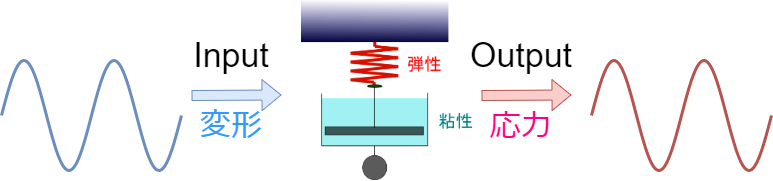
\includegraphics[width=.9\textwidth]{dynamic_ViscoElast_2.png}
		
% 	\begin{alertblock}{測定時のポイント}
% 		\begin{itemize}
% 			\item この枠組みは、線形応答となることが前提
% 			\item それを満たすために、微小ひずみを入力する。
% 		\end{itemize}
% 	\end{alertblock}
% \end{frame}

% \begin{frame}
% 	\frametitle{非線形応答でのLissajous}
% 		\begin{alertblock}{過大なひずみ $\Leftrightarrow$ 非線形応答}
% 			\centering
% 			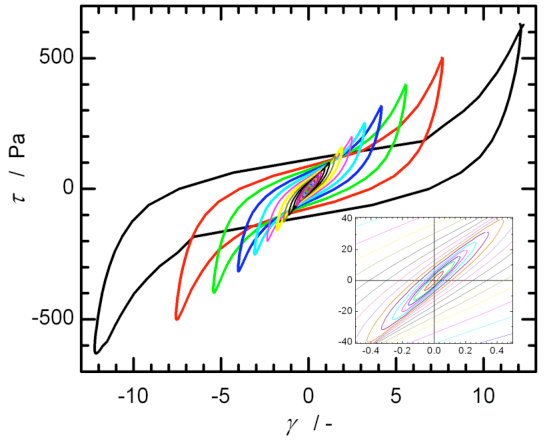
\includegraphics[width=.7\textwidth]{nonlinear_liss.png}	
% 		\end{alertblock}
% \end{frame}

% \begin{frame}
% 	\frametitle{ひずみ依存性}
% 		\begin{block}{貯蔵弾性率 $G^{\prime}$ のひずみ振幅 $\gamma_0$ 依存性}
% 			\begin{itemize}
% 				\item ひずみが過大となった非線形領域では、
% 				\begin{itemize}
% 					\item 高調波成分が無視できなくなり、 
% 					\item $G^{\prime}$ は線形応答から逸脱。
% 				\end{itemize}
% 			\end{itemize}
% 			\vspace{2mm}
% 			\centering
% 				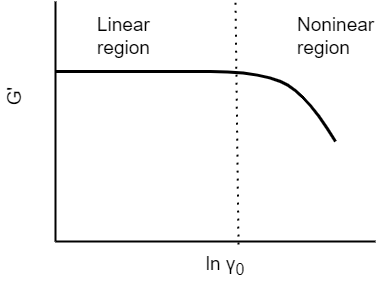
\includegraphics[width=.55\textwidth]{non-linear.png}
% 		\end{block}
% \end{frame}

% \begin{frame}
% 	\frametitle{動的な刺激への応答についてのまとめ}
%         \begin{boxnote}
%             \vspace{-3mm}
%             \begin{itemize}
%                 \item 動的な刺激と評価
%                     \begin{itemize}
%                         \item 動的な刺激(ひずみ)は周期的に時間変化
%                         \item 応答の周期は同一だが振幅、位相が異なる
%                     \end{itemize} 
%                 \item 動的な刺激への応答
%                     \begin{itemize}
%                         \item 弾性固体は同位相、粘性液体は位相が $\pi$/2 進む
%                         \item 粘弾性体は位相が少し($<\pi$/2 )進んだ応答
%                     \end{itemize} 
%                 \item 動的粘弾性測定とは
%                     \begin{itemize}
%                         \item 角周波数、ひずみ量、温度が測定パラメタ
%                         \item 貯蔵弾性率、損失弾性率、損失正接が出力
%                         \item 線形応答となるようにひずみ量に注意
%                     \end{itemize}
%             \end{itemize}
%         \end{boxnote}
% \end{frame}

% \section{粘弾性スペクトルについて}

% \subsection{粘弾性スペクトル}
% \begin{frame}
% 	\frametitle{粘弾性スペクトルとは}
% 	\begin{itemize}
% 		\item スペクトルとは?
% 		\begin{itemize}
% 			\item 複雑な情報や信号をその成分に分解し、成分ごとの大小にしたがって配列したもの
% 			\item 2次元以上で図示されることが多く、その図自体のことをスペクトルと呼ぶこともある。
% 			\item 一般には、光の波長ごとの強度分布を記述した分光スペクトルを指す場合が多い。
% 		\end{itemize}
% 		\item 粘弾性においては
% 		\begin{itemize}
% 			\item 信号である貯蔵および損失弾性率を、周波数や温度で展開した形の二次元で示される。
% 			\item 慣例として、展開したものによる分散という表現が用いられる。
% 			\item 前項のひずみ量を変化させたものをひずみ分散と呼ぶ。
% 		\end{itemize}
% 	\end{itemize}
% \end{frame}

% \subsection{動的測定と緩和の関係}
% \begin{frame}
% 	\frametitle{マックスウェルモデルに動的刺激を入れると}
% 		\begin{columns}[c, onlytextwidth]
% 			\column{.4\linewidth}
% 				\vspace{3mm}
% 				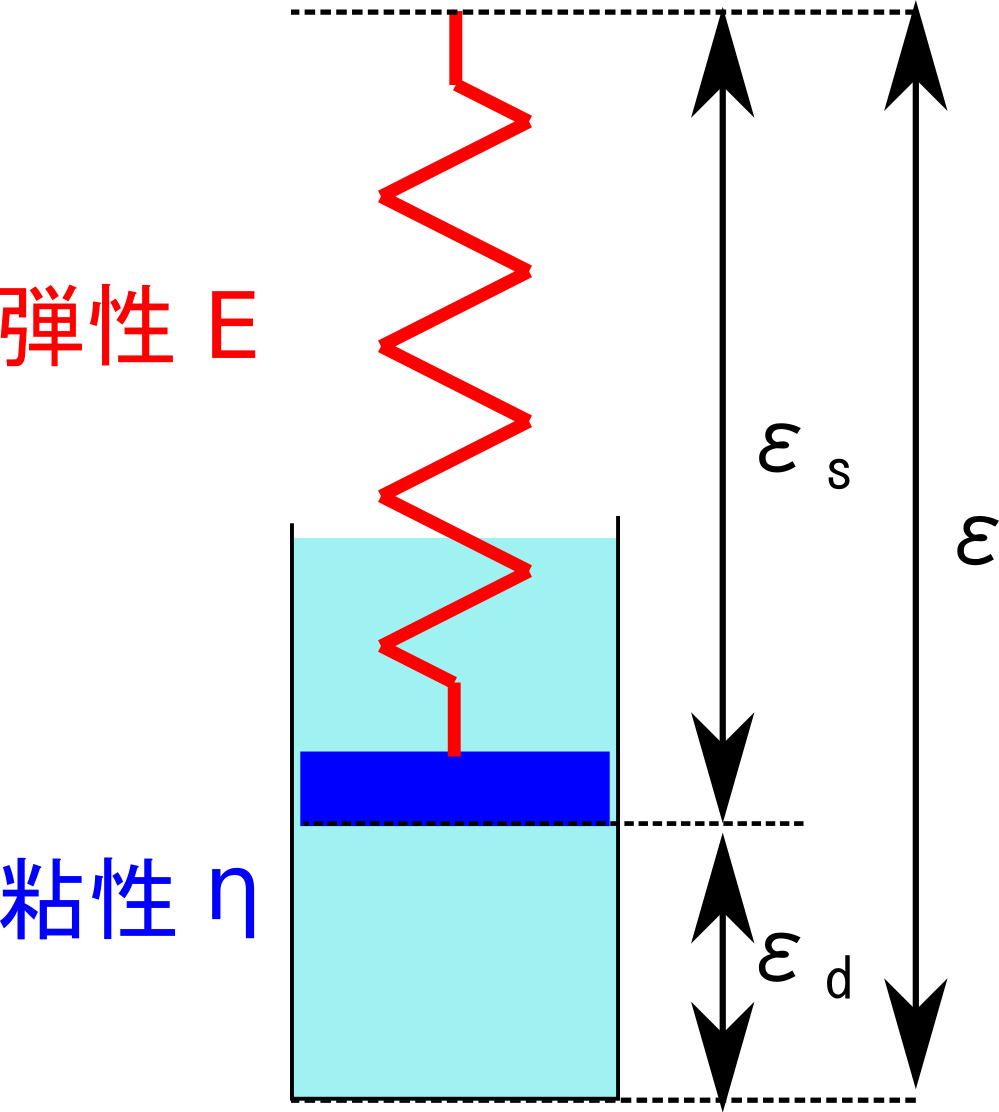
\includegraphics[width=.9\textwidth]{Maxwell_model.png}
% 				% \vspace{-3mm}
% 				\begin{align*}
% 					\begin{cases}
% 						\sigma = \sigma_s = \sigma_d \\
% 						\varepsilon = \varepsilon_s + \varepsilon_d
% 					\end{cases}
% 				\end{align*}
% 			\column{.55\linewidth}
% 				\begin{block}{マックスウェルモデルの応答}
% 					\alert{以下の導出の詳細は省略}
% 					\begin{itemize}
% 						\item 応力応答の一般式は
% 						\vspace{-3mm}
% 						\begin{align*}
% 							\sigma(t) = \sigma_0 \exp \left( - \dfrac{t}{\tau} \right)
% 						\end{align*}
% 						\item \vspace{-3mm}
% 						\item 角周波数 $\omega$ の動的ひずみを入れると
% 						\vspace{-3mm}
% 						\begin{align*}
% 							\begin{cases}
% 								G^{\prime}(\omega) = G\dfrac{\omega^2 \tau^2}{1+\omega^2\tau^2} \\[12pt]
% 								G^{\prime \prime}(\omega) = G\dfrac{\omega \tau}{1+\omega^2\tau^2}
% 							\end{cases}
% 						\end{align*}
% 					\end{itemize}		
% 				\end{block}
% 		\end{columns}
% \end{frame}

% \begin{frame}
% 	\frametitle{動的測定と緩和の関係}
% 		\vspace{-3mm}
% 		\begin{columns}[c, onlytextwidth]
% 			\column{.42\linewidth}
% 				% \begin{block}{マックスウェルモデルの応答}
% 					\centering
% 					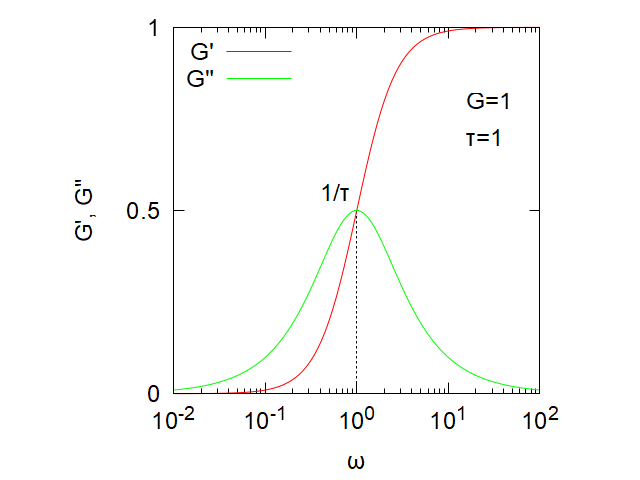
\includegraphics[width=\textwidth]{maxwell_dynamic.png}

% 					\vspace{-5mm}
% 					\begin{align*}
% 						\begin{cases}
% 							G^{\prime}(\omega) = G\dfrac{\omega^2 \tau^2}{1+\omega^2\tau^2} \\[12pt]
% 							G^{\prime \prime}(\omega) = G\dfrac{\omega \tau}{1+\omega^2\tau^2}
% 						\end{cases}
% 					\end{align*}
% 				% \end{block}
				
% 				% \vspace{-3mm}
% 			\column{.58\linewidth}
% 				\begin{alertblock}{弾性率の周波数依存性}
% 					\begin{itemize}
% 						\item 高周波数では
% 						\begin{itemize}
% 							\item 貯蔵弾性率 $G^{\prime}$ が主
% 							\item ほぼ弾性的な応答
% 						\end{itemize}
% 						\item 低周波数では
% 						\begin{itemize}
% 							\item 双方ともに小さい
% 							\item 応力は発生しない
% 						\end{itemize}
% 						\item 緩和時間に対応する角周波数\\($\omega=1/\tau$) で
% 						\begin{itemize}
% 							\item 損失弾性率 $G^{\prime\prime}$ が極大
% 							\item 緩和に伴うエネルギー散逸が最大化
% 						\end{itemize}
% 					\end{itemize}
% 				\end{alertblock}
% 		\end{columns}

% 		\vspace{3mm}
% 		\large
% 		\centering
% 		\alert{緩和の過程で損失弾性率 $G^{\prime\prime}$ が極大を示す。}
% \end{frame}

% \subsection{温度分散と周波数分散}
% \begin{frame}
% 	\frametitle{温度分散と周波数分散}
% 		\vspace{-5mm}
% 	\begin{columns}[T, onlytextwidth]
% 		\column{.38\linewidth}
% 			\begin{exampleblock}{変更可能なパラメタ}
% 				\begin{itemize}
% 				\item 角周波数 $\omega$
% 				\item ひずみ量 $\gamma$
% 				\item 測定温度 $T$
% 				\end{itemize}
% 			\end{exampleblock}
% 		\column{.58\linewidth}
% 			\begin{block}{測定できる物性値}
% 				\begin{itemize}
% 				\item 貯蔵弾性率 $G^{\prime}$ :弾性的挙動
% 				\item 損失弾性率 $G^{\prime \prime}$ :粘性的挙動
% 				\item 損失正接 $\tan \delta$ :粘性の寄与
% 				\end{itemize}
% 			\end{block}
% 	\end{columns}

% 		\vspace{3mm}
% 			\centering
% 				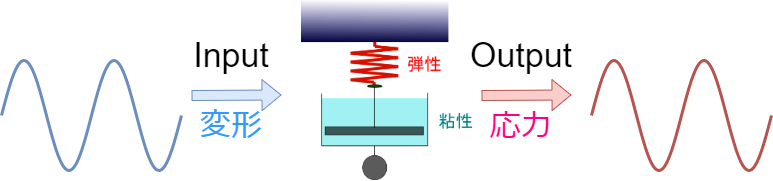
\includegraphics[width=.9\textwidth]{dynamic_ViscoElast_2.png}
		
% 	\begin{alertblock}{二種類の分散測定}
% 		\begin{itemize}
% 			\item 測定温度を段階的に変化させて、一定周波数で測定
% 			\item 任意の温度で、周波数を変化させて測定。
% 		\end{itemize}
% 	\end{alertblock}
% \end{frame}

% % \subsection{温度分散}
% \begin{frame}
%     \frametitle{温度分散とは}
% 			% \begin{block}{温度分散とは}
% 				\begin{itemize}
% 					\item \alert{任意の周波数で温度を変数}として動的粘弾性を測定
% 					\item \alert{低温での高い貯蔵弾性率が温度上昇で単調減少}
% 					\item 温度変化で生じる物質の硬化・軟化挙動には有用
% 					\item 一般に、得られる情報が曖昧になりがち。
% 				\end{itemize}

% 				\vspace{2mm}
% 				\centering
% 				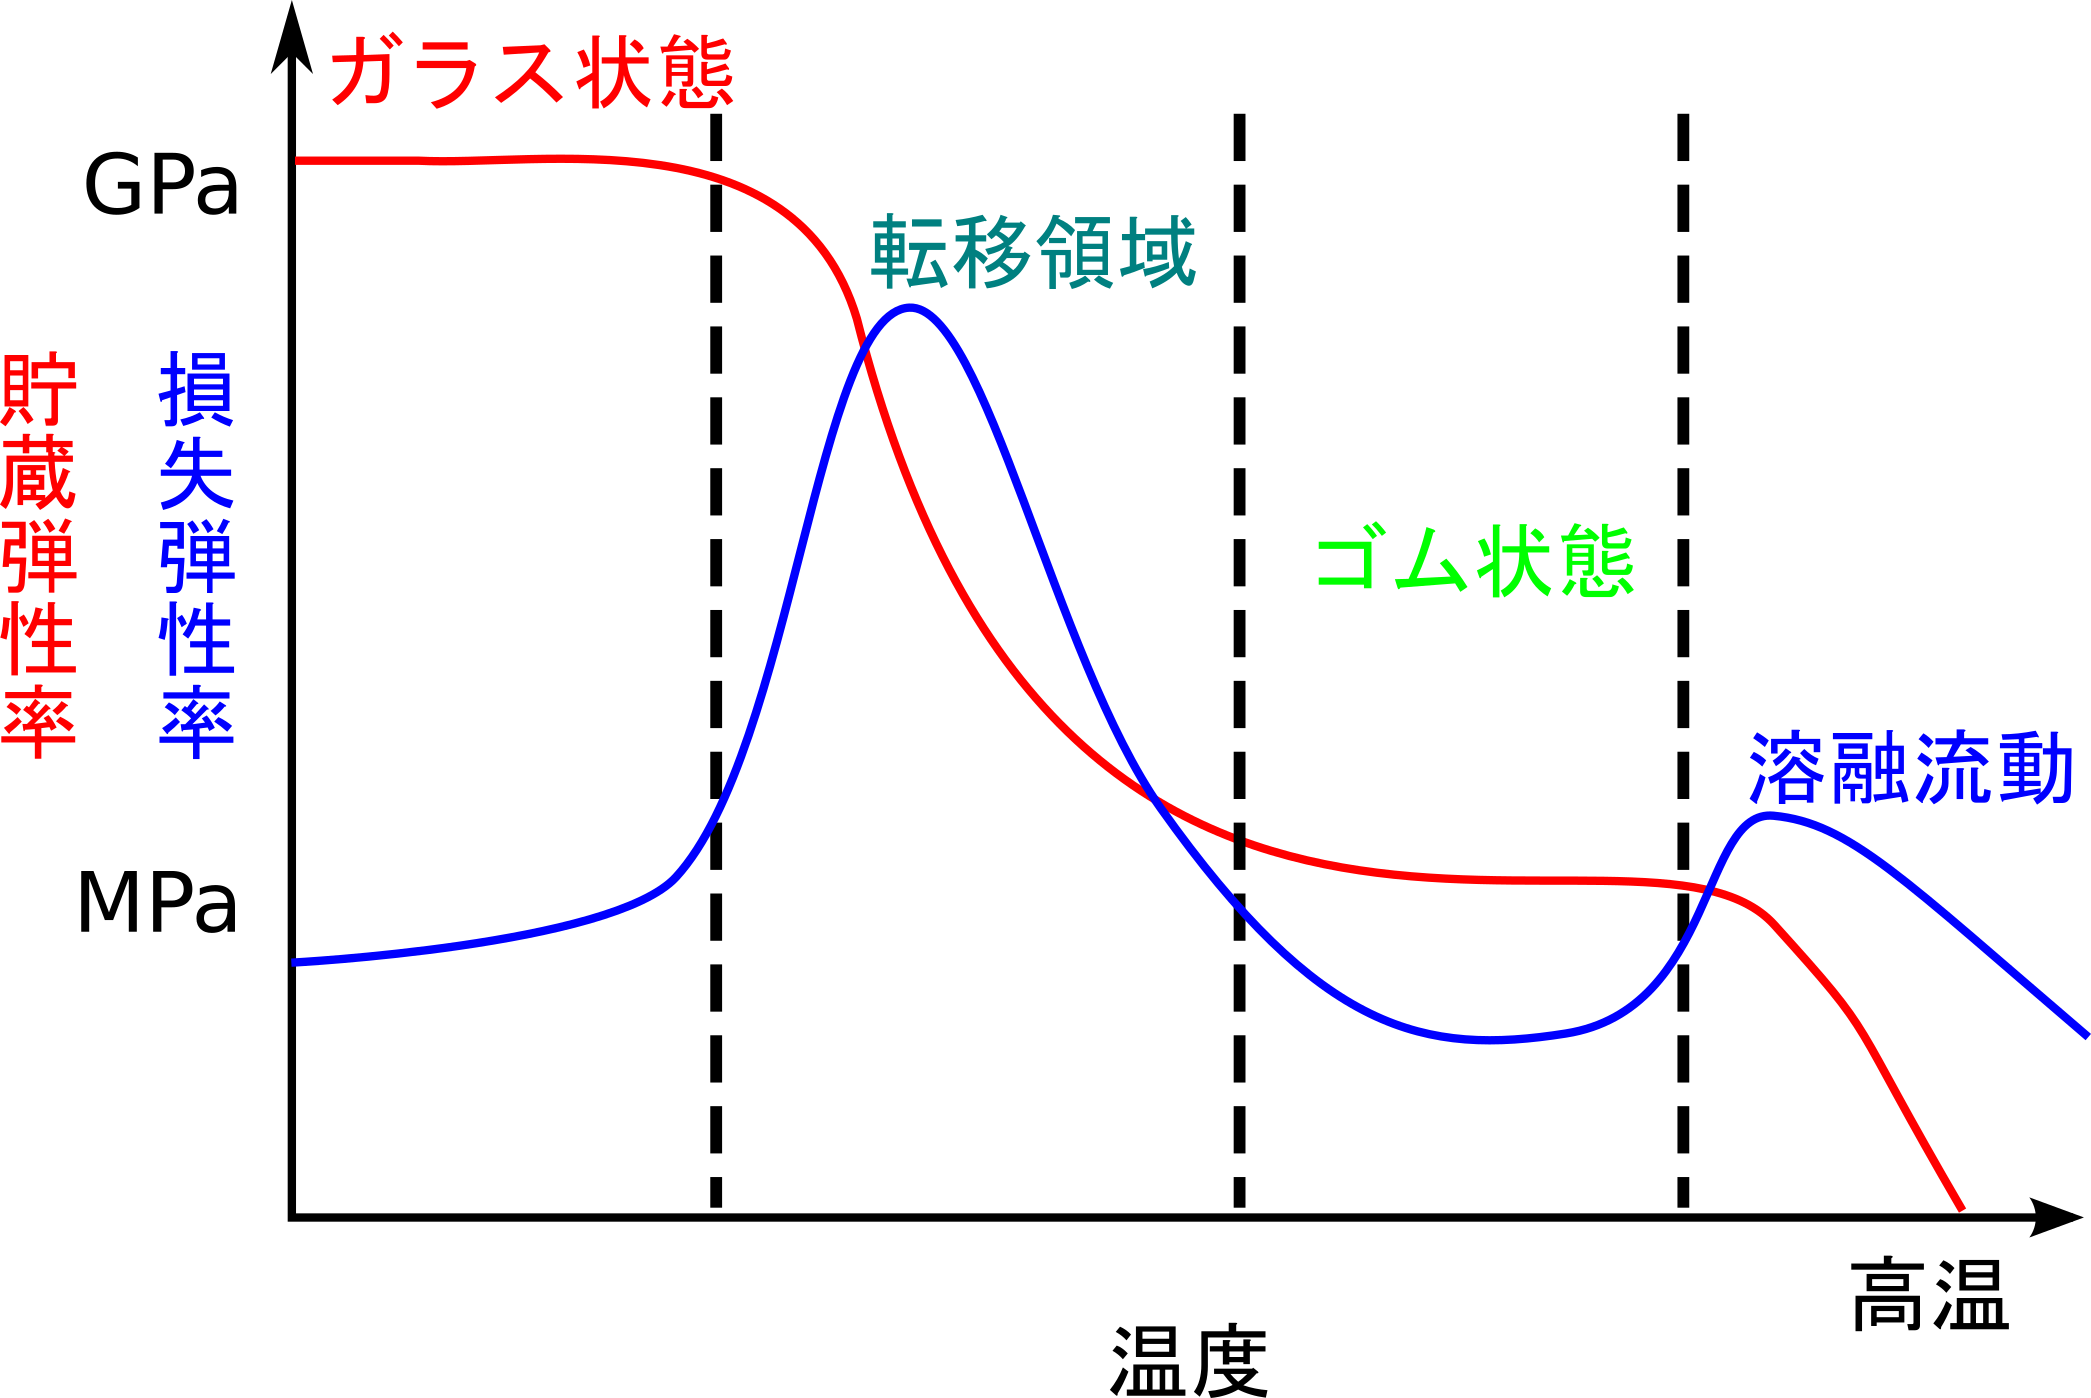
\includegraphics[width=.7\textwidth]{dynamic_ViscoElast_Temp.png}
% 			% \end{block}
			
% \end{frame}

% % \subsection{周波数分散}
% \begin{frame}
%     \frametitle{周波数分散とは}
% 		\begin{itemize}
% 			\item \alert{任意の温度で周波数を変数}として粘弾性スペクトル
% 			% \item 高周波数での高い貯蔵弾性率が低周波数で単調減少
% 			\item \alert{温度分散を左右反転したような形に注意}
% 					\begin{itemize}
%                         \item 低温は高周波(短時間)の振る舞いに相当
%                     \end{itemize}
% 			\item 内部状態の推定に有用な情報を得られる場合が多い
% 		\end{itemize}

% 		\vspace{2mm}
% 		\centering
% 		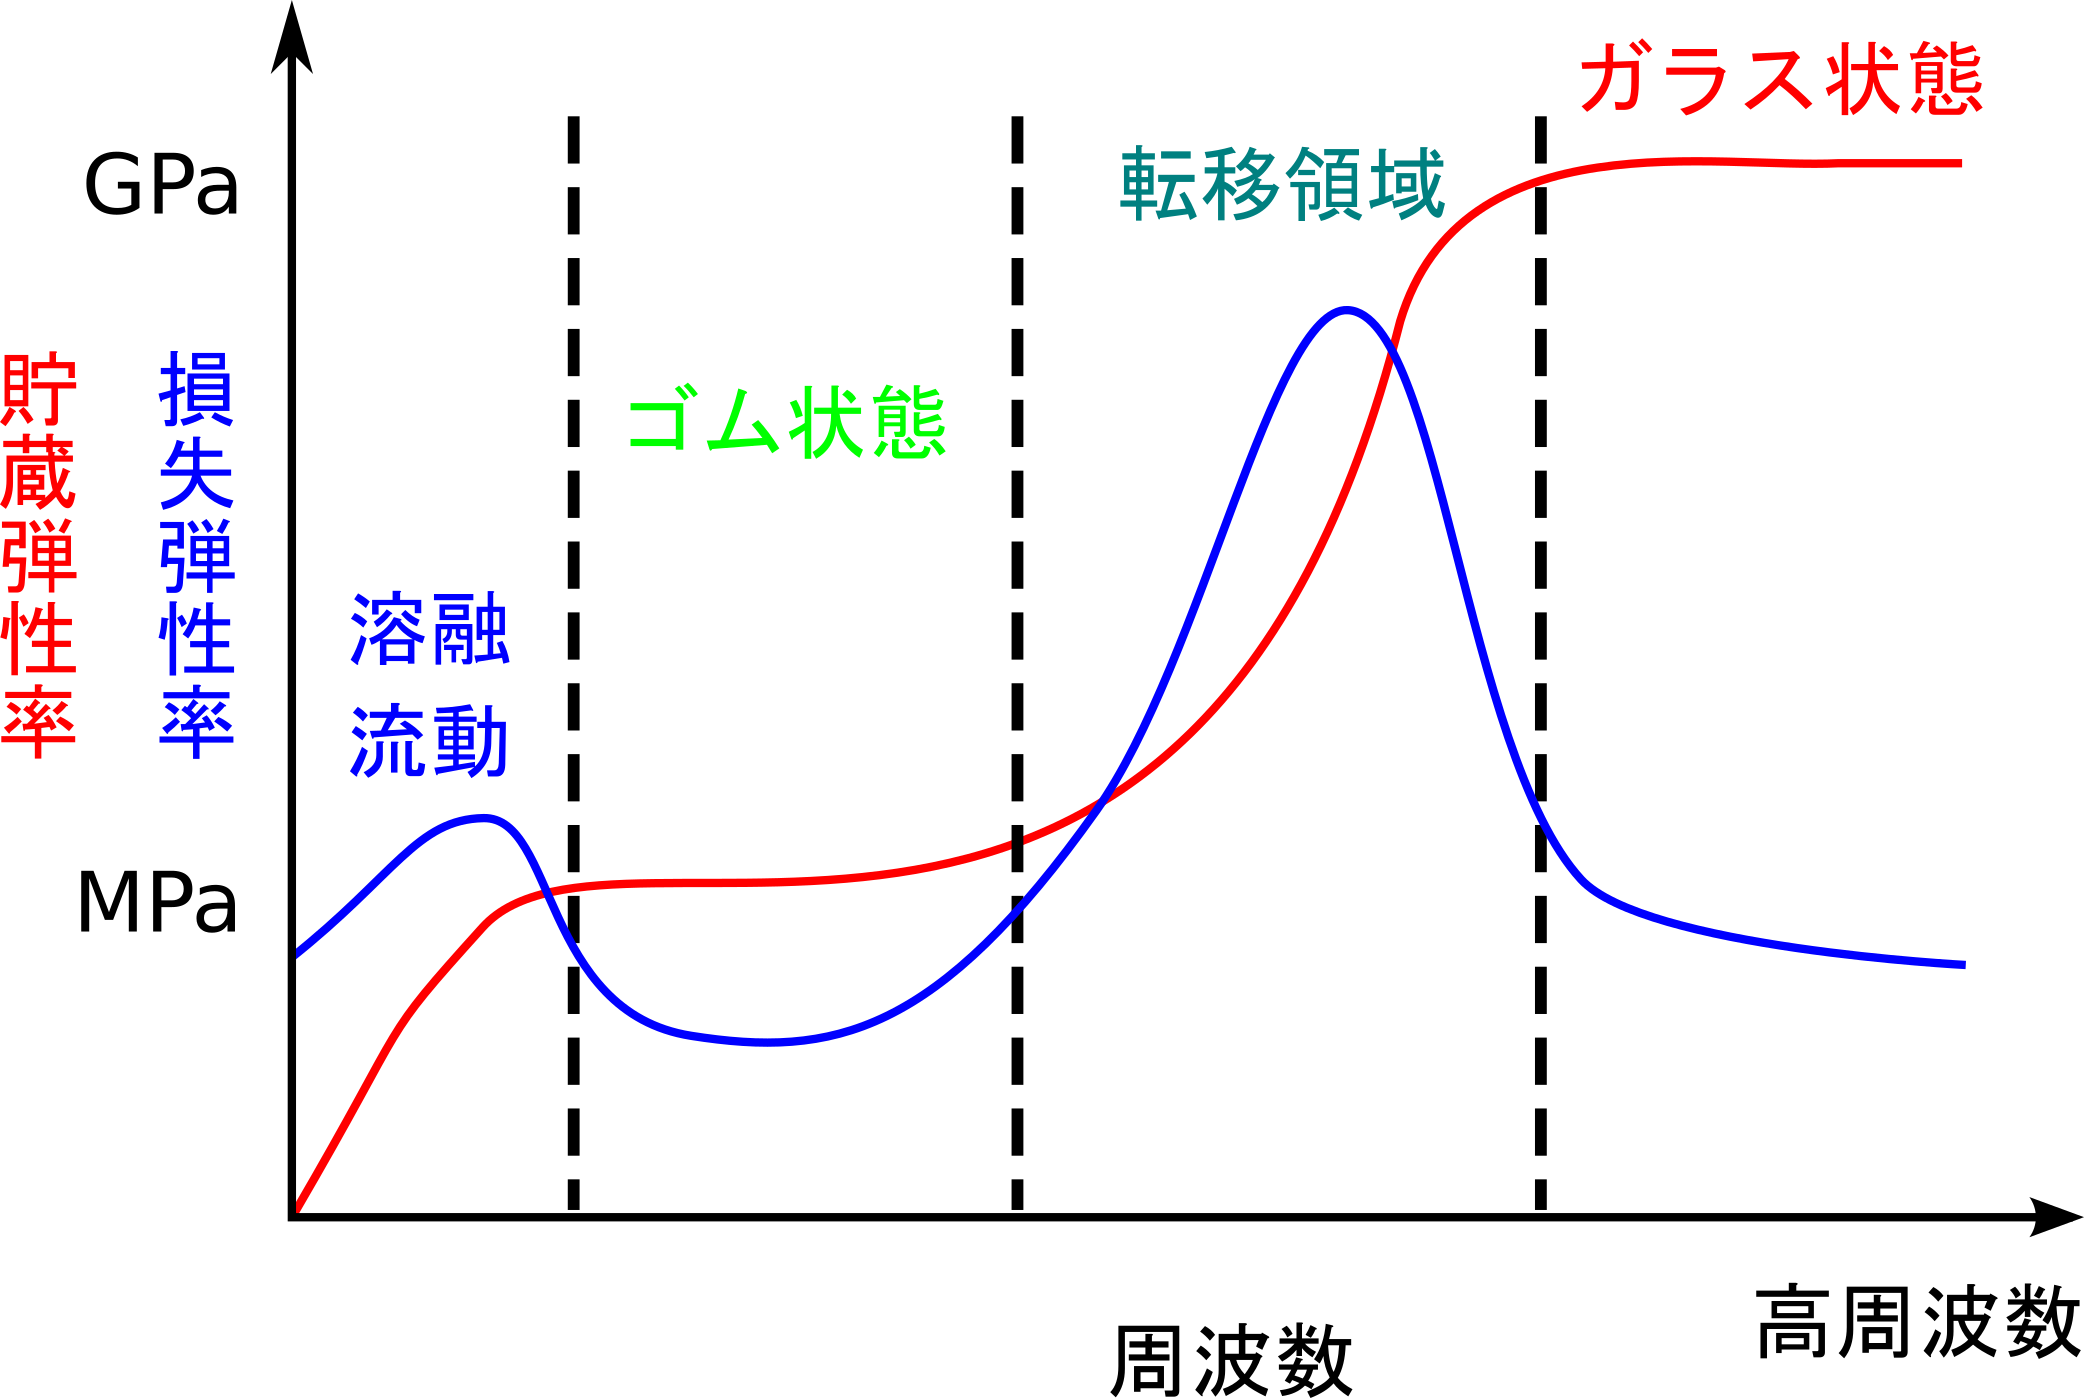
\includegraphics[width=.7\textwidth]{dynamic_ViscoElast_Freq.png}
% \end{frame}

% \begin{frame}
% 	\frametitle{粘弾性スペクトルについてのまとめ}
%         \begin{boxnote}
%             \vspace{-3mm}
%             \begin{itemize}
%                 \item 粘弾性スペクトルとは
%                     \begin{itemize}
%                         \item スペクトルは光の波長等の入力で展開した図
%                         \item 粘弾性測定では、温度や周波数で展開する
%                     \end{itemize} 
%                 \item 動的測定と緩和の関係
%                     \begin{itemize}
%                         \item マックスウェルモデルで解析すると、
%                         \begin{itemize}
% 							\item 貯蔵弾性率 $G^{\prime}$ は周波数低下で単調減少
% 							\item 緩和時間 $\omega = 1/\tau$ で損失弾性率 $G^{\prime\prime}$ が極大
% 						\end{itemize}
%                     \end{itemize} 
%                 \item 温度分散と周波数分散
%                     \begin{itemize}
%                         \item 温度分散で貯蔵弾性率 $G^{\prime}$ は高温で単調減少
%                         \item 転移領域で損失弾性率が極大
%                         \item 低い温度が高周波数、高温が低周波数に対応
%                     \end{itemize}
%             \end{itemize}
%         \end{boxnote}
% \end{frame}

\end{document}